% !TeX program = xelatex
% ============================================================
%  微网与外部电网电力调控策略
%  全国大学生数学建模竞赛 · 2026 C 题
%  编译: xelatex main.tex  (跑两遍以生成目录/交叉引用)
% ============================================================
\documentclass[12pt,a4paper]{article}

% ---------- 中文支持 ----------
% 使用 Windows 系统字体：宋体正文 / 黑体标题（ctex 自带 \heiti 等命令）
\usepackage[UTF8,scheme=plain,fontset=windows]{ctex}

% ---------- 页面：上下左右 ≥ 2.5cm ----------
\usepackage[top=2.4cm,bottom=2.4cm,left=2.7cm,right=2.7cm]{geometry}

% ---------- 数学 ----------
\usepackage{amsmath,amssymb,amsfonts,bm}
\usepackage{mathtools}

% ---------- 图表 ----------
\usepackage{graphicx}
\usepackage{float}
\usepackage{placeins}
\usepackage{verbatim}
\usepackage{subcaption}
\usepackage{booktabs}
\usepackage{multirow}
\usepackage{longtable}
\usepackage{array}
\usepackage{makecell}
\usepackage{tabularx}
\usepackage{tikz}
\usetikzlibrary{arrows.meta,positioning,shapes.geometric}
\graphicspath{{figs/}{figure_package/figures/}}

% ---------- 排版助手 ----------
\usepackage{enumitem}
\usepackage{caption}
\usepackage{titlesec}
\usepackage{fancyhdr}
\usepackage{setspace}
\usepackage{xcolor}
\usepackage[hidelinks]{hyperref}
\usepackage{siunitx}

% ---------- 版式参数 ----------
\linespread{1.12}                          % 行距
% 首行缩进两个汉字宽（\ccwd = 当前中文字符宽），段落间距为 0
\setlength{\parindent}{2\ccwd}
\setlength{\parskip}{0pt}
\captionsetup{font=small,labelsep=quad}
\numberwithin{equation}{section}
\numberwithin{figure}{section}
\numberwithin{table}{section}

% 标题样式：黑体
\titleformat{\section}{\heiti\zihao{3}}{\thesection}{1em}{}
\titleformat{\subsection}{\heiti\zihao{4}}{\thesubsection}{1em}{}
\titleformat{\subsubsection}{\heiti\zihao{-4}}{\thesubsubsection}{1em}{}
% 注意：这里必须用【不带星号】的 \titlespacing。
% 带星号的 \titlespacing* 会设置 \@afterindentfalse，
% 导致标题后紧跟的第一段取消首行缩进（本论文要求每段都缩进两格）。
\titlespacing{\section}{0pt}{1.4ex plus .2ex}{1.0ex plus .2ex}
\titlespacing{\subsection}{0pt}{1.2ex plus .2ex}{0.8ex plus .2ex}
\titlespacing{\subsubsection}{0pt}{1.0ex plus .2ex}{0.6ex plus .2ex}
% 双保险：显式要求标题后首段缩进
\makeatletter
\@afterindenttrue
\makeatother

% 页脚页码（居中）
\pagestyle{fancy}
\fancyhf{}
\renewcommand{\headrulewidth}{0pt}
\fancyfoot[C]{\thepage}

% 常用记号
\newcommand{\dd}{\mathrm{d}}
\newcommand{\E}{\mathbb{E}}
\newcommand{\Prob}{\mathbb{P}}
\newcommand{\kw}{\,\text{kWh}}
\newcommand{\yuan}{\,\text{元}}
\newcommand{\argmin}{\operatorname*{arg\,min}}

% ============================================================
\begin{document}

% ---------------- 摘要页 ----------------
% ==================== 摘要专用页 ====================
\begin{center}
  {\heiti\zihao{2} 微网与外部电网电力调控策略}
\end{center}

\vspace{0.6em}

\noindent{\heiti\zihao{4} 摘\quad 要}

\vspace{0.3em}

本文针对微网在光伏本地消纳与外网购电成本之间的权衡问题，围绕\textbf{储能设备的优化调度}，
建立了一套由确定性到随机、由单时点到多时点的递进式数学模型，并给出四问的完整求解结果。
全文统一采用 10 分钟为时段（一天 144 段），储能容量 $[1200,10800]$ kWh、
单向效率 $0.9$、功率上限 $5000$ kW，不售电且允许弃光，缺口按 5 倍电价紧急购电。

\textbf{问题一}为典型日确定性调度。以全天购电费最小为目标，建立含 720 个决策变量的
稀疏线性规划（LP），用 HiGHS 求解。我们证明了\textbf{该 LP 的松弛是紧的}：当往返效率
$0.9^2=0.81<1$ 时，若某时段同时充电与放电，则可构造等 SOC 扰动使购电量严格下降，
故最优解自动满足充放电互斥，\textbf{无需引入二元变量}。求解得全天最优购电费
\textbf{35\,126.95 元}，较无储能基线 48\,052.05 元\textbf{节省 26.90\%}；其中光伏余电消纳贡献
6\,727.28 元、峰谷价差套利贡献 6\,197.82 元，两者几乎各占一半。

\textbf{问题二}为全年滚动随机日前调度。我们首先识别出本题的\textbf{报童型结构}：计划购电量照付
（缺货成本为 0、过量成本为电价 $p$），而缺额须按 $5p$ 补救，故临界分位
$F^*=c_u/(c_o+c_u)=0.80$，即计划量应取净负载的 \textbf{80\% 分位}而非均值。据此建立
\textbf{两阶段随机规划}：用「计划净供给 $\ge$ 点预测」的不等式约束叠加历史残差场景的紧急购电
兜底，配合 48 小时前瞻窗口逐日滚动。预测严格只用历史数据（负载：最近 4 次同星期均值
$+$ 近 5 日残差漂移；光伏：近 7 日均值 $+$ 近 28 日残差漂移）。关键改进是
\textbf{剔除 1 月 1--7 日的回退预测残差}（该 7 天负载内核缺少同星期历史，口径与后续不一致），
以 56 天等权残差构造场景，全年总费用 \textbf{1\,438.91 万元}。

\textbf{问题三}引入 0/6/12/18 点的光伏发布预报与多时点调整机制。首先将题面「计划量高于调整量
部分按 50\% 违约电价、调整量高于计划量部分按 1.5 倍」的计费规则统一为
$J=\sum_t[p_tg_t^0+1.5p_tu_t-0.5p_tv_t+5p_te_t]$，并指出\textbf{调减项的系数必须为 $-0.5p$}
（净省 $0.5p$）——否则最优解永不调整，题目失去意义。其次提出\textbf{在线预报融合}：
以历史预测 $H$ 与发布预报 $F$ 的因果最小二乘权重 $\alpha$ 融合，并做收缩偏差校正。
进而构建\textbf{经验场景树}：把历史日在后续发布时刻的预报修订作为未来信息做二叉聚类，
\textbf{节点内共享购电/充放电/SOC 变量}，从而在变量结构上严格保证非前视。
全年费用 \textbf{1\,402.24 万元}，较同口径基线\textbf{节省 2.55\%}，紧急购电量减少 28.74\%。
边际分析表明 6 点与 12 点调整各贡献约 8 万元，\textbf{18 点几乎无额外收益}。
进一步通过完美预见下界（1\,223.16 万元）与权重饱和性检验等 30 余组对照，
说明该方案在给定数据与已测试模型族内已接近性能上界。

\textbf{问题四}考虑实时波动电价。对 4-2，我们保留「当天 0 点电价未知」的主模型，
以 1 月历史选定「最近 4 次同星期几均值」为电价预测器，并构造
\textbf{电价—净负载联合场景}（同一历史日的两种残差配对），
理由是 $\E[p_t(N_t-z_t)_+]\neq\E[p_t]\E[(N_t-z_t)_+]$——高电价可能与缺电同时发生，
不能分解。全年费用 \textbf{1\,516.30 万元}。对 4-3，在 4-2 上叠加多时点调整与预报融合机制，
费用进一步降至 \textbf{1\,506.17 万元}。对比可见\textbf{波动电价下多时点调整的价值
（约 10.1 万元）显著大于固定电价下的价值（约 1.5 万元）}，说明电价波动放大了调整机制的价值。

\vspace{0.4em}
\noindent{\heiti 关键词：}\quad 储能优化调度；线性规划；报童模型；两阶段随机规划；
滚动时域优化；预报融合；场景树；联合场景

\vspace{0.8em}
\noindent\rule{\textwidth}{0.4pt}


% ---------------- 正文 ----------------
% 页码连续编号：摘要为第 1 页，正文从第 2 页起依次递增，不重置。
\newpage

% ==================== 一、问题重述与分析 ====================
\section{问题重述与分析}

\subsection{问题背景}

微网是为解决光伏等分布式能源本地消纳、减少并网问题而发展起来的小型发用电系统。
出于经济性考虑，\textbf{非孤岛式微网}可在外部电网（下称外网）电价较低、或分布式能源有剩余电量时
为储能设备充电，并在外网电价较高时释放储存的电能，从而降低购电成本。
因此，如何在光伏出力不确定、电价时变的条件下制定\textbf{购电与充放电策略}，
是微网经济运行的核心问题。

本文研究的微网含光伏发电与储能设备，配置如下（题附录 1）：
最大容量 $12000\kw$，最大充放电功率 $5000$ kW，电量须保持在 $[1200,\ 10800]\kw$，
充放电单向效率均为 $90\%$，$2025$ 年 $1$ 月 $1$ 日 $0$:00 初始电量为 $6000\kw$。
微网不得向外网售电；微网供电不足时须向外网\textbf{紧急购电}，电价为交易时刻电价的 $5$ 倍。

\subsection{数据说明}

\begin{table}[H]
\centering
\caption{附件数据汇总}
\label{tab:data}
\small
\begin{tabularx}{\textwidth}{@{}c l X c@{}}
\toprule
附件 & 内容 & 用途 & 时间粒度 \\
\midrule
1 & 某天 144 段的电价、小区负载、光伏发电预测功率 & 问题一全部；二/三问的电价与预测回退 & 10 min \\
2 & 2025.1.1--12.31 每天的实际负载与光伏实际功率 & 二/三/四问的预测与结算 & 10 min \\
3 & 每日 $0$、$6$、$12$、$18$ 时发布的未来 24 h 整点光伏预报 & 三问、四之 4-3 的调整依据 & 1 h（整点）\\
4 & 2025.1.1--12.31 每天不同时间的电价 & 四问的结算电价 & 10 min \\
5 & 结果文件模板 & 各问 \texttt{result*.xlsx} 格式 & — \\
\bottomrule
\end{tabularx}
\end{table}

\subsection{统一口径约定}

为避免四问之间混淆，全文采用以下一致口径，后续各问不再重复声明。

\begin{enumerate}[itemsep=2pt,topsep=3pt]
  \item \textbf{时段划分}：一天划分为 $T=144$ 个时段，每段时长 $\Delta t=\tfrac{1}{6}$ h。
        附件中负载、光伏功率的单位为 kW，须乘以 $\Delta t$ 折算为每段电量（kWh）。
  \item \textbf{时间标签}：附件中的时刻为\textbf{区间末}时刻，即 \texttt{00:10} 表示 00:00--00:10，
        \texttt{0:00+1} 表示当天 24:00。
  \item \textbf{储能约束}：储电量 $E_t\in[1200,\ 10800]$；每段充、放电量
        $c_t,d_t\le 5000\Delta t=833.33\kw$；效率递推为
        $E_t=E_{t-1}+0.9c_t-d_t/0.9$。
  \item \textbf{交易规则}：不外送电；允许弃光与弃置多余的计划购电；缺口按 $5$ 倍电价紧急购电。
\end{enumerate}

\subsection{四问的递进关系}

四问在不确定性维度上层层递进，构成一条完整的建模主线：

\begin{center}
\begin{tabular}{@{}c c c c@{}}
\toprule
问题 & 电价 & 光伏信息 & 决策时点 \\
\midrule
问题一 & 已知（典型日）   & 已知              & 单时点（日内一次）\\
问题二 & 每日固定         & 仅历史预测        & 仅 $0$:00 \\
问题三 & 每日固定         & 历史预测 $+$ 发布预报 & $0/6/12/18$ 时 \\
问题四 & \textbf{实时波动} & 历史预测 $+$ 发布预报 & 4-2：仅 $0$:00；4-3：$0/6/12/18$ 时 \\
\bottomrule
\end{tabular}
\end{center}

相应地，模型从\textbf{确定性 LP}（问题一）过渡到\textbf{两阶段随机规划}（问题二），
再到\textbf{多阶段场景树随机规划}（问题三），最后引入\textbf{电价随机性}形成
双重不确定下的联合场景模型（问题四）。

\subsection{本文的主要特色}

\begin{enumerate}[itemsep=2pt,topsep=3pt]
  \item \textbf{报童结构的识别}：指出问题二的本质是报童问题，临界分位 $F^*=0.80$，
        为计划购电量提供了清晰的经济学解释，而非盲目调参。
  \item \textbf{LP 松弛紧性的严格证明}：证明问题一无需充放电互斥的二元约束，
        大幅降低计算复杂度（见 \S\ref{sec:q1-tight}）。
  \item \textbf{计费规则的统一化建模}：把问题三的分段计费规则写成单一线性表达式，
        并给出系数符号的必要性论证（见 \S\ref{sec:q3-fee}）。
  \item \textbf{场景树保证非前视}：节点内共享控制变量，使模型在结构上不可能"偷看"未来信息。
  \item \textbf{电价—净负载联合场景}：识别出期望不可分解性
        $\E[p\cdot(N-z)_+]\neq\E[p]\E[(N-z)_+]$，据此构造配对场景。
\end{enumerate}

% ==================== 二、模型假设、符号与前提 ====================
\section{模型假设与符号约定}

\subsection{模型假设}

本文的建模基于以下假设。为便于评阅，每条假设均给出理由。

\begin{enumerate}[label=\textbf{A\arabic*.},itemsep=4pt,topsep=4pt,leftmargin=*]
  \item \textbf{段内功率恒定。}
        附件提供的负载、光伏数据以 10 分钟为间隔，本文视其为该区间内的平均功率，
        段内功率恒定，故每段电量 $=$ 功率 $\times \Delta t$。
        \emph{理由}：题面只给出离散采样点，采用平均功率是对连续量的标准离散化处理，
        且与附件 1 的“某天不同时间的电价/负载”表述一致。

  \item \textbf{储能效率模型为单向恒定效率。}
        充电效率与放电效率均为 $0.9$（往返 $0.81$），不计及功率相关性、
        温度效应与循环老化衰减。
        \emph{理由}：题附录 1 明确给出“充放电效率为 $90\%$”，
        未提供效率曲线或衰减规律，故采用题给常值。
        题面未区分“单向”与“往返”，本文在 \S\ref{sec:eff-robust} 给出两口径的完整对照。

  \item \textbf{不计储能折旧与运维费用。}
        目标函数中只包含购电相关费用。
        \emph{理由}：题面要求最小化购电费用，未提及设备成本；
        引入未经给定的折旧率反而会带来主观偏差。

  \item \textbf{严格因果性（非前视）。}
        任何决策（包括预测器的构造、融合权重的估计、场景的提取与场景树的分支）
        均只使用决策时刻之前\textbf{已实现}的数据，不得读取当天及未来的实际值。
        \emph{理由}：这是滚动决策问题可行性的前提，也是所有对照实验公平比较的基础。
        本文在问题一至问题四\textbf{逐问强化}该原则：问题一为全信息已知；
        问题二要求预测只依赖历史；问题三进一步要求场景树的节点划分也只能依据
        届时新发布的预报（\S\ref{sec:q3-nonanticip}）；问题四再加电价的非前视。

  \item \textbf{电价按供电时段计价。}
        每段费用 $=$ 该段的电价 $\times$ 该段的购电量，
        而不是按“作出决策的时刻”统一计价。
        \emph{理由}：物理上电量的计量发生在用电时刻；
        这使问题三的四个发布时刻各自对应一组时段价格，
        避免了把所有未来时段折算到决策时刻价格的非常规设定。

  \item \textbf{储能充放电互斥（但不显式约束）。}
        物理上储能不能同时充放电。本文\textbf{不加入二元变量}，
        而是证明在本文的模型结构下最优解自动满足互斥（\S\ref{sec:q1-tight}），
        并在输出前逐段检查。
        \emph{理由}：见 \S\ref{sec:q1-tight} 的等价性证明。
\end{enumerate}

\noindent 题面已明确给定的计费与物理规则（计划购电照付、取消部分退还原价并另付
$50\%$ 违约费、增购按 $1.5$ 倍、紧急购电按 $5$ 倍、不外送电且允许弃光、
各问的终端电量要求）不属于假设，而是\textbf{建模的已知条件}，
其统一处理见 \S\ref{sec:conventions}；与各问模型直接相关的终端条件
在对应问题的模型建立中陈述。

\subsection{全局符号说明}
\label{sec:notation}

四问共用同一套物理量，故统一在模型假设后集中说明，各问不再重复定义。
表 \ref{tab:notation} 给出全文使用的符号。

\begin{table}[H]
\centering
\caption{全文符号说明（四问通用）}
\label{tab:notation}
\small
\begin{tabularx}{\textwidth}{@{}c l X c@{}}
\toprule
符号 & 含义 & 说明 & 单位 \\
\midrule
\multicolumn{4}{@{}l}{\textit{（一）时段与数据}}\\
\midrule
$T$            & 时段数                   & 一天划分为 $T=144$ 个十分钟时段 & — \\
$\Delta t$     & 每段时长                 & $\Delta t=1/6$ h & h \\
$t$            & 时段索引                 & $t=1,\dots,144$ & — \\
$d$            & 日期索引                 & 年度模型中的日 & — \\
$p_t$          & 第 $t$ 段电价             & 问题一至三用附件 1；问题四用附件 4 & 元/kWh \\
$L_t$          & 第 $t$ 段负载电量         & 附件中为功率，乘 $\Delta t$ 折算 & kWh \\
$V_t$          & 第 $t$ 段光伏发电量       & 同上 & kWh \\
$N_t$          & 净负载                   & $N_t=L_t-V_t$ & kWh \\
\midrule
\multicolumn{4}{@{}l}{\textit{（二）决策变量}}\\
\midrule
$g_t$          & 计划购电量               & 日前制定的购电量 & kWh \\
$g_t^{0}$      & 0 点原计划购电量          & 问题三、4-3 的初始计划 & kWh \\
$q_t$          & 最终调整后购电量          & 问题三、4-3 的执行量 & kWh \\
$c_t$          & 充电量                   & 作用于设备外端 & kWh \\
$d_t$          & 放电量                   & 作用于设备外端 & kWh \\
$w_t$          & 弃光量                   & 仅设非负约束，见 \S\ref{sec:q1-model} & kWh \\
$E_t$          & 段末储能电量             & 内部库存，$E_t\in[1200,\,10800]$ & kWh \\
$u_t,v_t$      & 相对原计划的增购量、减购量 & $u_t=(q_t-g_t^0)_+$，$v_t=(g_t^0-q_t)_+$ & kWh \\
$e_t$          & 紧急购电量               & 缺口补救，按 $5p_t$ 计价 & kWh \\
\midrule
\multicolumn{4}{@{}l}{\textit{（三）效率与储能参数}}\\
\midrule
$\eta_c,\eta_d$ & 充电效率、放电效率       & 主口径 $\eta_c=\eta_d=0.9$，往返 $0.81$ & — \\
$\rho$         & 往返效率                 & $\rho=\eta_c\eta_d$ & — \\
$E_0$          & 初始储电量               & 题给 2025-01-01 0:00 为 6000 & kWh \\
\midrule
\multicolumn{4}{@{}l}{\textit{（四）随机规划量}}\\
\midrule
$\hat N_t$     & 净负载点预测             & 只用历史数据构造 & kWh \\
$N_{s,t}$      & 场景净负载               & 场景 $s$ 的第 $t$ 段净负载 & kWh \\
$p_{s,t}$      & 场景电价                 & 仅问题四使用 & 元/kWh \\
$s$            & 场景索引                 & 由历史日整日残差构成 & — \\
$w_s$          & 场景权重                 & 等权时 $w_s=1/S$ & — \\
$n$            & 场景树节点索引           & 问题三、4-3 & — \\
$\pi_n$        & 节点概率                 & 落入该节点的历史日数占比 & — \\
$\alpha$       & 融合权重                 & 在线估计，见 \S\ref{sec:q3-fusion} & — \\
\midrule
\multicolumn{4}{@{}l}{\textit{（五）评价指标}}\\
\midrule
$J$            & 总费用                   & 分项构成见对应公式 & 元 \\
$\lambda_t$    & 边际电价（对偶变量）     & 能量平衡约束的影子价格 & 元/kWh \\
\bottomrule
\end{tabularx}
\end{table}

\noindent 记号说明：$(\cdot)_+=\max\{\cdot,0\}$；$\E[\cdot]$ 为数学期望；
带下标 $s$ 的量表示随场景变化、由对应的历史日产生。
为避免与日期索引 $d$ 混淆，全文用 $d_t$ 表示放电量（与主程序中的变量名一致）。

% ==================== 三、问题一 ====================
\section{问题一：典型日确定性储能调度}

\subsection{问题分析}

问题一给定某典型日的电价、小区负载与光伏发电预测功率，要求制定使购电费最小的调度策略。
由于该日全部数据已知，这是一个\textbf{确定性优化问题}。

其经济本质是两条：
\begin{enumerate}[itemsep=2pt,topsep=3pt]
  \item \textbf{光伏余电消纳}：光伏出力超过负载时，若不储能则被迫弃光；
        储能可把余电存起来供后续使用，减少购电。
  \item \textbf{峰谷价差套利}：在低价时段多购电存入电池，在高价时段放电使用，
        赚取价差。能否套利取决于价差是否超过往返效率损失。
\end{enumerate}

\subsection{符号说明}

本问使用的全部符号已在 \S\ref{sec:notation} 表 \ref{tab:notation} 统一说明，此处不再重复。
下面直接给出模型。

\subsection{模型建立}
\label{sec:q1-model}

以全天购电费用最小为目标：

\begin{equation}
\min\ J_1=\sum_{t=1}^{144} p_t g_t
\label{eq:q1-obj}
\end{equation}

约束条件包括五组：

\textbf{(1) 功率平衡}（供给侧 $=$ 需求侧）：
\begin{equation}
g_t+V_t+d_t=L_t+c_t+w_t
\label{eq:q1-balance}
\end{equation}
其中 $w_t$ 为弃光量，故外购电与光伏之和，加上电池放电，恰好满足负载与电池充电。

\textbf{(2) 弃光非负}：
\begin{equation}
w_t\ge 0
\end{equation}
弃光量只设非负约束，\textbf{不显式添加} $w_t\le V_t$ 的上界。由等式平衡
$w_t=g_t+d_t-c_t-(L_t-V_t)$；目标只惩罚购电量，若最优解出现 $w_t>V_t$
（即净供给超过负载），令 $g_t\leftarrow g_t-\delta$、$w_t\leftarrow w_t-\delta$
可保持平衡不变而费用严格下降（对任意 $p_t>0$），与最优性矛盾。
因此最优解自动满足 $w_t\le V_t$，该上界冗余；省略它与第二、三问对松弛变量的
口径保持一致。本节末的约束核验同时报告“弃光非负”（属模型约束）与
“弃光未超光伏出力”（属本实例的数值观察，本实例弃光量为零）。

\textbf{(3) 储能电量递推}（注意充电乘效率、放电除效率）：
\begin{equation}
E_t=E_{t-1}+0.9\,c_t-\frac{d_t}{0.9},\qquad t=1,\dots,144
\label{eq:q1-soc}
\end{equation}

\textbf{(4) 储能容量与功率约束}：
\begin{equation}
1200\le E_t\le 10800,\qquad 0\le c_t\le \frac{5000}{6},\qquad 0\le d_t\le \frac{5000}{6}
\end{equation}

\textbf{(5) 非负与循环条件}：
\begin{equation}
g_t\ge 0,\qquad E_0=E_{144}=6000
\label{eq:q1-cycle}
\end{equation}

模型共含 $5\times 144=720$ 个决策变量，全部约束为线性，
构成一个稀疏线性规划（LP），调用 \texttt{scipy.optimize.linprog}（HiGHS 内点/单纯形）求解。

\subsection{关键性质：LP 松弛的紧性证明}
\label{sec:q1-tight}

物理上储能不能同时充电与放电，即要求 $c_t\cdot d_t=0$。
但引入这类互斥条件需要二元变量，问题变为混合整数规划（MILP），规模与计算量显著上升。
我们证明：\textbf{在本模型结构下，最优解自动满足互斥，无需显式约束}。

\begin{quote}
\textbf{命题。} 设某时段同时有 $c_t>0$ 与 $d_t>0$。取
\[
\varepsilon=\min\Bigl\{c_t,\ 0.81\,d_t,\ \frac{g_t}{0.19}\Bigr\}>0,
\]
并作替换 $c_t\leftarrow c_t-\varepsilon$、$d_t\leftarrow d_t-0.81\varepsilon$，其余变量不变。则
\begin{enumerate}[label=(\roman*),itemsep=1pt,topsep=2pt]
  \item \textbf{储电量轨迹与全部 SOC 约束完全不变}，因为
    \[
    0.9(c_t-\varepsilon)-\frac{d_t-0.81\varepsilon}{0.9}
    =\Bigl(0.9c_t-\frac{d_t}{0.9}\Bigr)-0.9\varepsilon+0.9\varepsilon
    =\Bigl(0.9c_t-\frac{d_t}{0.9}\Bigr);
    \]
  \item \textbf{充电、放电功率均不增加}（故功率约束仍满足）；
  \item 由功率平衡 \eqref{eq:q1-balance}，$g_t$ 变为 $g_t-0.19\varepsilon<g_t$，
        即\textbf{购电量严格下降}，费用随之严格下降。
\end{enumerate}
这与最优性矛盾。故最优解中必不存在“该时段有购电且同时充放电”的情形。
\end{quote}

\textbf{经济解释}：往返效率 $0.81<1$ 意味着“买 1 度电只有 0.81 度能存进电池再取出”。
当该时段仍在从外网购电时，把充放电的这部分对冲掉，等价于\textbf{少买一点电、同时少损耗一点}，
而负载供应不受影响——因此必然更省钱。

\textbf{验证}：本实例中 LP 最优解的 144 个时段\textbf{全部满足 $c_td_t=0$}，
无需任何后处理，故 LP 松弛是紧的。求解 MILP 作为对照，两者目标值完全相同
（$35\,126.95$ 元，差 $0.000000$），从数值上证实了上述证明。

\subsection{求解结果}

\begin{table}[H]
\centering
\caption{问题一求解结果对比}
\label{tab:q1-result}
\begin{tabular}{@{}l r r@{}}
\toprule
方案 & {购电费（元）} & {相对基线} \\
\midrule
无储能基线 & 48052.05 & — \\
\textbf{储能在位、优化调度} & \bfseries 35126.95 & \bfseries $-26.90\%$ \\
\bottomrule
\end{tabular}
\end{table}

经济性校验：充电加权均价 $0.4930$ 元/kWh，放电加权均价 $1.1376$ 元/kWh，
比值 $2.31$，高于盈亏平衡点 $1/0.81=1.235$，故储能套利有正收益。

\subsection{收益来源分解}

把优化结果与无储能基线逐项对比，可把 $12\,925.10$ 元的节省\textbf{严格分解}为两部分。
由逐时段功率平衡 $g_t=L_t+c_t-d_t-V_t+w_t$，
基线取 $c=d=0$ 且\ $w_t=\max(V_t-L_t,0)$，可得\textbf{严格恒等式}

\begin{equation}
\sum_t p_t\max(L_t-V_t,0)-\sum_t p_tg_t
=\sum_t p_t\max(V_t-L_t,0)+\sum_t p_td_t-\sum_t p_tc_t.
\label{eq:q1-decomp}
\end{equation}

即“总节省 $=$ 弃光消除 $+$ 净套利”，左端为基线购电费与优化购电费之差，
右端两项分别对应\textbf{被吸收的光伏余电价值}与\textbf{储能低买高卖的净收益}。
两者的经济含义见下表，\textbf{各项之和恒等于总节省，无重复、无遗漏}。

\begin{table}[H]
\centering
\small
\caption{问题一收益来源分解（严格恒等式 \eqref{eq:q1-decomp}）}
\label{tab:q1-gain}
\begin{tabularx}{\textwidth}{@{}l r r X@{}}
\toprule
收益来源 & {金额（元）} & {占基线} & 说明 \\
\midrule
光伏余电消纳 & 4037.75 & 8.40\% & 基线中被弃掉的 $6247.96\kw$ 全部被电池吸收 \\
峰谷价差套利 & 8887.35 & 18.50\% & 低价购电存入、高价放出，已扣除充电成本 \\
\midrule
\textbf{合计} & \bfseries 12925.10 & \bfseries 26.90\% & \\
\bottomrule
\end{tabularx}
\end{table}

可见\textbf{套利是主要来源（约 69\%），消纳次之（约 31\%）}。
这是因为本例中光伏余电仅 $6247.96\kw$（占光伏总量 $11.3\%$），
而峰谷价差最高达 $1.40/0.37\approx 3.8$ 倍，远超往返效率盈亏平衡点 $1/0.81=1.235$，
故储能的边际价值主要体现在跨时段搬移电量而非吸收余电。

\subsection{电量平衡与调度解释}

\begin{table}[H]
\centering
\caption{问题一全天电量平衡}
\begin{tabular}{@{}l r l r@{}}
\toprule
项目 & {电量（kWh）} & 项目 & {电量（kWh）} \\
\midrule
外网购电   & 59482.70 & 小区负载     & 111024.81 \\
光伏发电   & 55482.84 & 电池充电     & 20740.67 \\
电池放电   & 16799.94 & 弃光         & \bfseries 0.00 \\
         &          & 电池往返损失 & 3940.73 \\
\bottomrule
\end{tabular}
\end{table}

\textbf{为何弃光为 0？}光伏总量 $55\,482.84\kw$ 全部被利用，
其中一部分直接供给负载、一部分存入电池。这说明在本日的“光伏—负载—电价”组合下，
电池容量足以吸收全部余电，储能的边际价值主要体现在套利而非消纳。

\textbf{为何充放电发生在这些时段？}附件 1 的电价并非简单的“两段式”，
而是呈现\textbf{三段特征}：

\begin{table}[H]
\centering
\caption{典型日电价的时段结构}
\begin{tabular}{@{}l l l@{}}
\toprule
时段 & 电价水平（元/kWh） & 调度行为 \\
\midrule
凌晨 $0$--$6$ 时   & 低谷 $0.37$--$0.44$ & 大量充电（$0$--$4$ 时充 $4500\kw$）\\
上午 $6$--$9$ 时    & \textbf{尖峰}，最高 $1.01$  & 放电供负载 \\
中午 $10$--$16$ 时   & 回落 $0.41$--$0.53$   & 光伏余电 + 补充电 \\
傍晚 $18$--$20$ 时   & \textbf{全天最高} $1.35$--$1.40$ & 放电（$16$--$20$ 时放 $5780\kw$）\\
\bottomrule
\end{tabular}
\end{table}

调度的全部逻辑围绕这三段展开：在凌晨与中午的低价窗口充电，
在上午与傍晚的两个高价窗口放电，从而最大化价差收益。

\subsection{对偶分析}

对功率平衡约束 \eqref{eq:q1-balance} 取对偶变量（影子价格）$\lambda_t$，
其经济含义为“第 $t$ 段若能多供 1 kWh，购电费能下降多少”。
由最优性条件，$\lambda_t\le p_t$ 时该段不购电（$g_t=0$）；
$\lambda_t=p_t$ 时该段购电为正。对偶量可用来识别“哪些时段的容量瓶颈最值钱”，
具体数值已保存于结果文件的 \texttt{duals.npz} 中。

\begin{figure}[htbp]
\centering
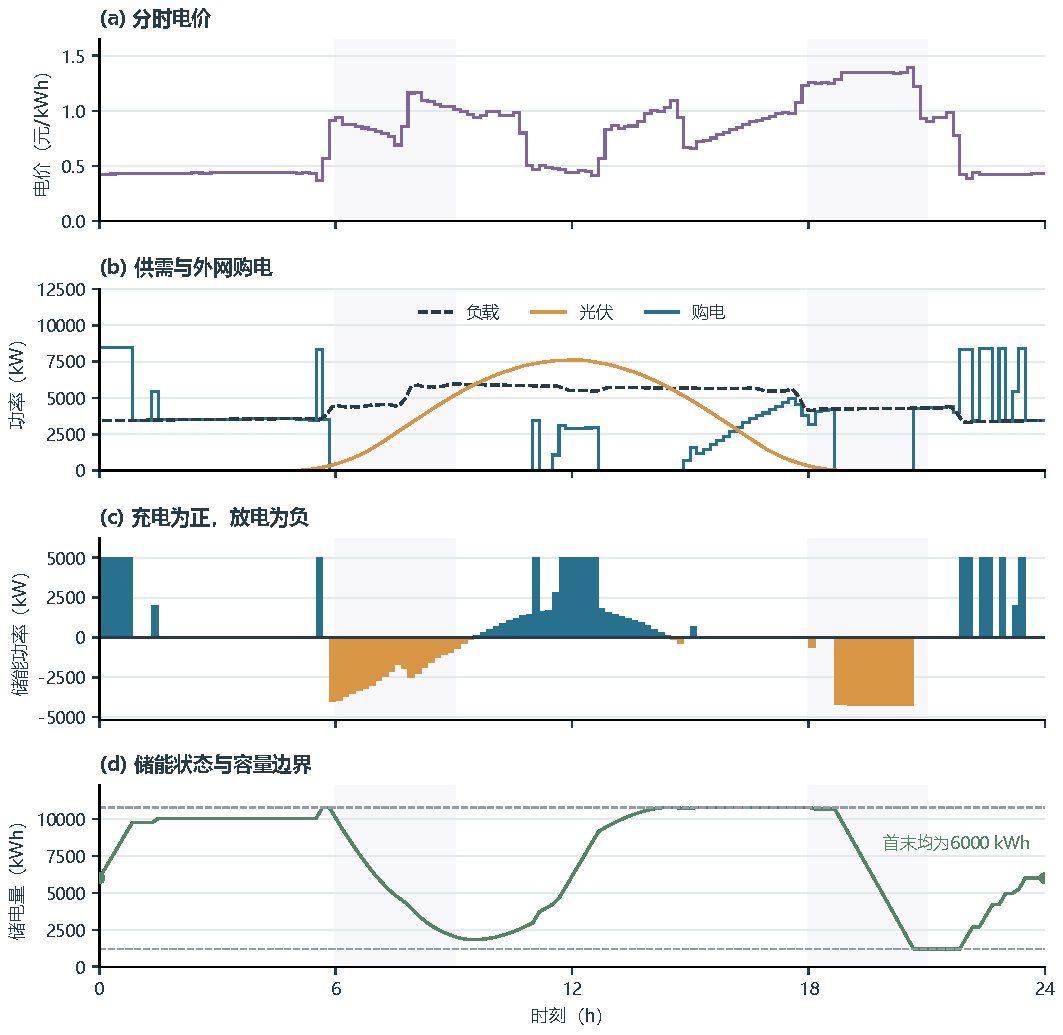
\includegraphics[width=0.95\textwidth]{01_q1_dispatch.pdf}
\caption{典型日确定性调度结果。四个面板共享时间轴，依次展示电价、供需与购电功率、
储能充放电功率及储电量；水平虚线为 1200 与 10800 kWh 的储电量边界，
浅色背景仅辅助定位早晚时段。}
\label{fig:q1-dispatch}
\end{figure}

储电量始终位于规定区间内，且日初、日末均为 6000 kWh，
因此该收益并非通过消耗日初库存获得。

\begin{figure}[htbp]
\centering
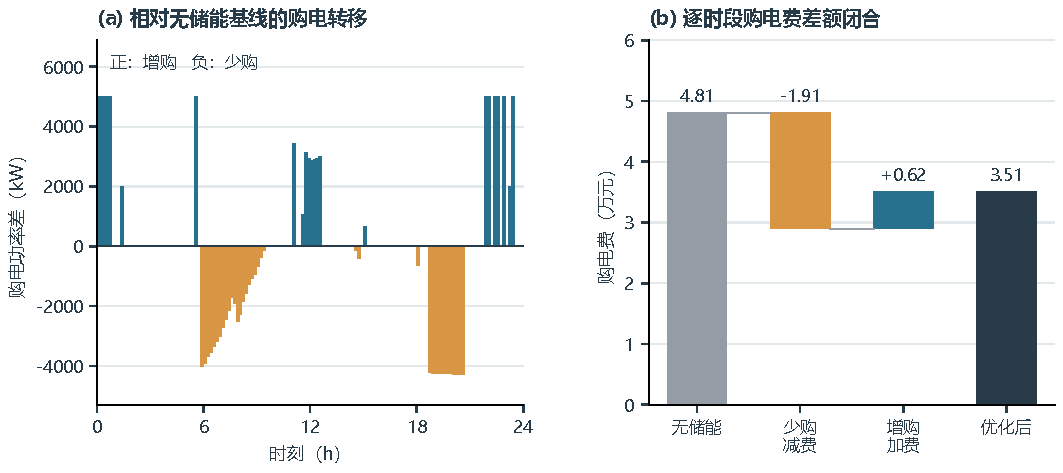
\includegraphics[width=0.95\textwidth]{02_q1_savings.pdf}
\caption{储能调度相对无储能基线的购电差异与费用桥接。左图为优化购电功率
减去无储能购电功率；右图按同一时段电价分别累计少购所减少的费用和增购所增加的费用。}
\label{fig:q1-savings}
\end{figure}

图 \ref{fig:q1-savings} 给出了节省的账面来源：储能使部分时段少购电，
对应费用减少 $19\,111.64$ 元；同时在另一些时段增购电，对应费用增加 $6\,186.54$ 元。
两者抵消后净节省 $12\,925.10$ 元，降幅为 $26.90\%$。
这一分解是逐时段购电费差额的恒等核算，图 \ref{fig:q1-gain} 的
$4037.75$ 元与 $8887.35$ 元则是按能量来源的另一组恒等分解，
两种口径各自自洽，不互相替代，也不把同一节省重复归因为独立效应。

\begin{figure}[H]
\centering
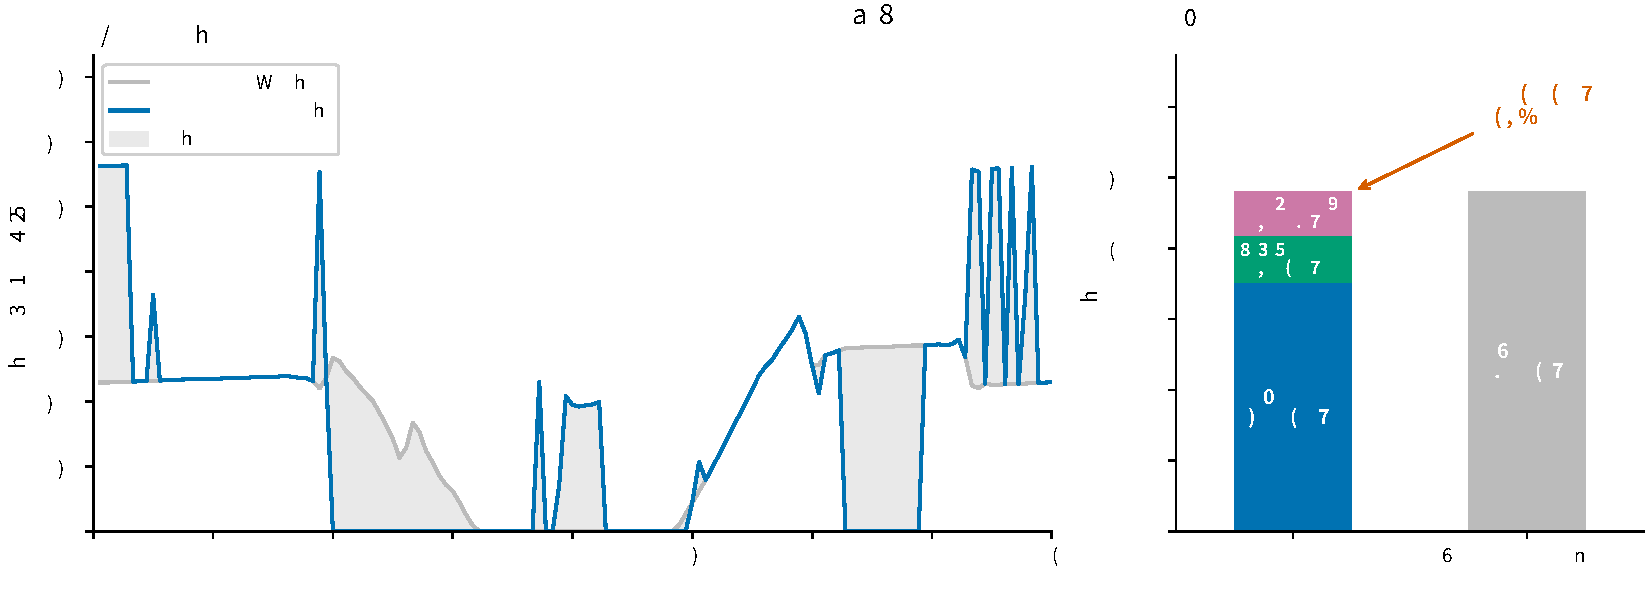
\includegraphics[width=0.95\textwidth]{q1_comparison.pdf}
\caption{问题一收益来源分解：弃光消除项与净套利项之和恒等于总节省
（式 \eqref{eq:q1-decomp}）}
\label{fig:q1-gain}
\end{figure}

\subsection{题目指定表格}

\begin{table}[H]
\centering
\caption{表 1\quad 微网在指定时间段的购电量及全天购电量与购电费}
\begin{tabular}{@{}l r r@{}}
\toprule
时间段 & {购电量（kWh）} & {该时段电价（元/kWh）} \\
\midrule
10:00--10:10 & 0.00   & 0.9919 \\
12:00--12:10 & 480.41 & 0.4411 \\
14:00--14:10 & 0.00   & 1.0002 \\
16:00--16:10 & 445.43 & 0.8271 \\
18:00--18:10 & 531.89 & 1.2561 \\
20:00--20:10 & 0.00   & 1.3513 \\
\midrule
\textbf{全天购电量} & \bfseries 59482.70 & \\
\textbf{全天购电费} & \bfseries 35126.95 元 & \\
\bottomrule
\end{tabular}
\end{table}

\begin{table}[H]
\centering
\caption{表 2\quad 储能设备在指定时间段的充放电量及 $0$:00 与 $24$:00 的储电量}
\begin{tabular}{@{}l r r@{}}
\toprule
时间段 & {充电量（kWh）} & {放电量（kWh）} \\
\midrule
0:00--4:00   & 4500.00 & 0.00 \\
4:00--8:00   & 833.33  & 6365.84 \\
8:00--12:00  & 4787.96 & 1703.00 \\
12:00--16:00 & 5286.04 & 91.10 \\
16:00--20:00 & 0.00    & 5780.13 \\
20:00--24:00 & 5333.33 & 2859.87 \\
\midrule
$0$:00 储电量  & \multicolumn{2}{c}{6000.00 kWh} \\
$24$:00 储电量 & \multicolumn{2}{c}{6000.00 kWh} \\
\bottomrule
\end{tabular}
\end{table}

% ==================== 四、问题二 ====================
\section{问题二：滚动随机日前调度}

\subsection{问题分析：报童结构的识别}

问题二在每天 $0$:00 制定当天的计划购电策略，而负载与光伏的实际值未知。
题面给出两条关键计费规则：

\begin{quote}
\textit{“微网提供的电能不可低于小区负载，如果低于负载，需向外网紧急购电，
其电价是交易时刻电价的 5 倍。除紧急购电费用外，其他时间段的购电费用均按计划购电量计算。”}
\end{quote}

第二条规则意味着：\textbf{计划购电量照付，用不完不退}。于是单时段决策呈现出典型的
\textbf{报童模型}结构：计划量过高的代价是“多付了钱”，边际成本为电价 $p$；
计划量过低的代价是“缺额须按 $5p$ 补救”，边际成本为 $4p$。最优计划量应满足临界分位数

\begin{equation}
F^*=\frac{c_u}{c_o+c_u}=\frac{4p}{p+4p}=\frac{4}{5}=0.80,
\label{eq:newsvendor}
\end{equation}

其中 $c_o=p$ 为过量成本，$c_u=4p$ 为缺货成本。\textbf{即计划购电量应取净负载分布的 80\% 分位，
而非期望值（50\% 分位）。}这一结论解释了为何“按点预测制定计划”会系统性低估购电量、
进而产生大量昂贵的紧急购电。

\begin{figure}[H]
\centering
\begin{tikzpicture}[scale=0.95,every node/.style={font=\small}]
  % 坐标轴
  \draw[->] (0,0) -- (7.2,0) node[right]{计划量 $g$};
  \draw[->] (0,0) -- (0,3.6) node[above]{成本};
  % 过量成本线
  \draw[thick,blue] (0,2.6) -- (3.4,0.9);
  \node[blue] at (1.6,2.35) {$c_o=p$ （多买）};
  % 缺货成本线
  \draw[thick,red] (3.4,0.9) -- (6.8,3.3);
  \node[red] at (5.5,2.9) {$c_u=4p$ （少买）};
  % 最优点
  \fill (3.4,0.9) circle (2.2pt);
  \draw[dashed] (3.4,0.9) -- (3.4,0) node[below]{$F^*=0.80$};
  \node at (3.4,0.35) {};
\end{tikzpicture}
\caption{报童结构示意：最优计划量位于 $80\%$ 分位，而非均值}
\label{fig:newsvendor}
\end{figure}

\subsection{两阶段随机规划模型}

设 $\hat N_t$ 为净负载点预测（kWh/段），$\{N_{s,t}\}_{s=1}^{S}$ 为历史残差构造的场景，
$w_s$ 为场景权重。每天在 48 h 窗口上求解如下两阶段随机规划：

\begin{equation}
\min\ J_2=\underbrace{\sum_{t\in 48h} p_tg_t}_{\text{计划购电费}}
+\underbrace{5\sum_{s}w_s\sum_{t\in \text{当天}} p_t\,e_{s,t}}_{\text{期望紧急购电费}}
\label{eq:q2-obj}
\end{equation}

约束为：

\begin{align}
&\text{（计划净供给下界）}\quad g_t+d_t-c_t\ \ge\ \hat N_t, \label{eq:q2-floor}\\
&\text{（场景缺口兜底）}\quad g_t+d_t-c_t+e_{s,t}\ \ge\ N_{s,t},\qquad e_{s,t}\ge 0, \label{eq:q2-scen}\\
&\text{（SOC 递推）}\quad E_t=E_{t-1}+0.9c_t-\frac{d_t}{0.9}, \label{eq:q2-soc}\\
&\text{（容量与功率）}\quad 1200\le E_t\le 10800,\quad 0\le c_t,d_t\le \frac{5000}{6},\quad g_t\ge0. \label{eq:q2-cap}
\end{align}

\noindent\textbf{模型解读：}
\begin{itemize}[itemsep=2pt,topsep=3pt]
  \item 约束 \eqref{eq:q2-floor} 是\textbf{不等式}而非等式：计划净供给不低于点预测即可，
        允许“多买”。这一点至关重要：它使计划量可以落在“80\% 分位”而非均值上，
        与 \eqref{eq:newsvendor} 的报童结论一致。
  \item 约束 \eqref{eq:q2-scen} 用场景 $s$ 的紧急购电 $e_{s,t}$ 兜底最坏情形，
        其代价系数为 $5p_t$。第一阶段的 $g,c,d$ 对所有场景共享，
        因此模型天然满足\textbf{非前视}要求。
\end{itemize}

\subsection{预测方法（严格因果）}
\label{sec:q2-forecast}

所有预测只使用决策日 $d$ 之前已实现的数据：

\begin{table}[H]
\centering
\caption{问题二的预测内核}
\begin{tabular}{@{}l l l@{}}
\toprule
分量 & 方法 & 参数 \\
\midrule
负载 & 最近 $k$ 次同星期几的均值 $+$ 近 $m$ 天残差漂移 & $k=4,\ m=5$ \\
光伏 & 近 $m$ 天均值 $+$ 近 $m'$ 天残差漂移 & $m=7,\ m'=28$ \\
\bottomrule
\end{tabular}
\end{table}

以负载为例，点预测为
\begin{equation}
\hat L_{d,t}=\underbrace{\frac{1}{|\mathcal W_d|}\sum_{i\in\mathcal W_d}L_{i,t}}_{\text{同星期几均值}}
+\underbrace{\frac{1}{5}\sum_{i=d-5}^{d-1}\bigl(L_{i,t}-\hat L_{i,t}\bigr)}_{\text{残差漂移校正}},
\qquad \mathcal W_d=\{d-7j: j=1,\dots,4,\ d-7j\ge0\}.
\end{equation}

加入漂移校正的原因：同星期几均值反映的是“典型水平”，
而最近几天的系统性偏差（如天气趋势）可用近期残差均值捕捉，从而提高点预测精度。

\subsection{场景构造与“有效残差”修正}
\label{sec:q2-scen}

场景采用\textbf{整日联合残差}（而非逐时段独立抽样），以保留日内时间相关性：
\begin{equation}
N_{s,t}=\hat N_{d,t}+r_{s,t},\qquad r_{s,t}=N_{s,t}^{\text{hist}}-\hat N_{s,t}^{\text{hist}},
\end{equation}
其中 $s$ 取最近 56 个已结束的历史日，\textbf{等权} $w_s=1/56$。

\noindent\textbf{关键改进：剔除回退期残差。}
负载内核依赖“同星期几”的历史，而 1 月 1--7 日不足一周，
此时只能使用附件 1 的典型日曲线作\textbf{回退预测}。
这类回退预测的误差口径与 1 月 8 日之后的正常预测\textbf{不一致}，
若一并纳入场景会污染残差分布。

为此，我们把场景历史的起点设为 $d\ge 7$（即 1 月 8 日）：

\begin{table}[H]
\centering
\caption{有效残差的样本量增长}
\begin{tabular}{@{}l c c@{}}
\toprule
日期 & 可用历史残差天数 & 说明 \\
\midrule
2 月 1 日 & 24 & 1 月 8--31 日 \\
\vdots & \vdots & 逐日增加 \\
3 月初起 & 56（上限） & 达到窗口上限后滚动 \\
\bottomrule
\end{tabular}
\end{table}

\begin{table}[H]
\centering
\caption{窗口与加权方案的对照实验（第二问）}
\label{tab:q2-abl}
\small
\begin{tabular}{@{}l r r r@{}}
\toprule
方法 & {总费用（元）} & {较基线（元）} & {紧急电量（kWh）} \\
\midrule
56 天等权（含回退残差）      & 14401996.98 &        & 237775.35 \\
56 天 / 半衰期 7 天          & 14444376.04 & $-42379.06$ & 258228.71 \\
56 天 / 半衰期 14 天         & 14404271.57 & $-2274.59$  & 244460.92 \\
56 天 / 半衰期 28 天         & 14391380.10 & $+10616.87$ & 237997.14 \\
28 天等权                    & 14443538.21 & $-41541.23$ & 250845.99 \\
42 天等权                    & 14407394.33 & $-5397.35$  & 241795.11 \\
\midrule
\textbf{56 天等权 + 有效残差} & \bfseries 14389135.08 & \bfseries $+12861.89$ & 246063.25 \\
\midrule
56 天 / 半衰期 28 天（有效残差） & 14390031.13 & $+896.04$ & 243038.84 \\
\bottomrule
\end{tabular}
\end{table}

\noindent\textbf{结论}：短窗口与指数加权\textbf{均无稳定收益}（多数反而变差），
而剔除回退残差带来 $12\,861.89$ 元的改善。
其中 $28$ 天半衰期在统计期的改善主要来自 2 月（$-12\,638.73$ 元），
3--12 月合计反而增加 $2\,021.86$ 元，说明它捕获的是\textbf{启动阶段效应}而非全年适应能力。

\begin{figure}[H]
\centering
\begin{tikzpicture}[scale=0.9,every node/.style={font=\small}]
  % 时间轴
  \draw[->] (0,0) -- (12,0) node[right]{天数 $d$};
  \foreach \x/\lab in {1.5/1, 3.5/7, 5.5/8, 8.5/56, 10.5/365} {
     \draw (\x,0.08) -- (\x,-0.08) node[below]{\lab};
  }
  % 回退期
  \fill[red!18] (0,0) rectangle (5.5,1.5);
  \node[red!70!black] at (2.7,0.75) {回退期（剔除）};
  % 有效残差期
  \fill[green!18] (5.5,0) rectangle (11.5,1.5);
  \node[green!45!black] at (8.6,0.75) {有效残差窗口（56 天滚动）};
  \draw[dashed] (5.5,0) -- (5.5,1.5);
\end{tikzpicture}
\caption{有效残差的时间口径：剔除 1 月 1--7 日的回退预测残差}
\label{fig:q2-residual}
\end{figure}

\subsection{滚动执行与终端条件}

每天在 48 小时窗口上求解，但\textbf{只执行前 24 小时}（当天 144 段），
次日重新求解。终端条件为\textbf{窗口末回到窗口起始电量}：
\begin{equation}
E_{288}=E_{\text{窗口起始}},
\end{equation}
而非每天日末回到日初。原因：滚动优化中终端条件代表“未来价值”，
若要求每天回到日初，会人为禁止跨日套利，系统性低估储能价值。

实际执行的紧急购电量为
\begin{equation}
e_{d,t}=\max\bigl\{N_{d,t}-g_{d,t}-d_{d,t}+c_{d,t},\ 0\bigr\},
\end{equation}
实际费用为
\begin{equation}
C=\sum_{d}\sum_t\bigl[p_tg_{d,t}+5p_te_{d,t}\bigr].
\end{equation}

\subsection{结果}

\begin{table}[H]
\centering
\caption{问题二最终结果（2 月 1 日--12 月 31 日，334 天）}
\label{tab:q2-final}
\begin{tabular}{@{}l r@{}}
\toprule
项目 & {金额（元）} \\
\midrule
计划购电费   & 13462061.30 \\
紧急购电费   & 927073.78 \\
\midrule
\textbf{总费用} & \bfseries 14389135.08 \\
\bottomrule
\end{tabular}
\end{table}

\noindent 全年计划购电量 $22\,098\,240.82\kw$，紧急购电量 $246\,063.25\kw$。
初始储电量 $8550\kw$（1 月预热后），年末回到 $6000\kw$。

\begin{figure}[H]
\centering
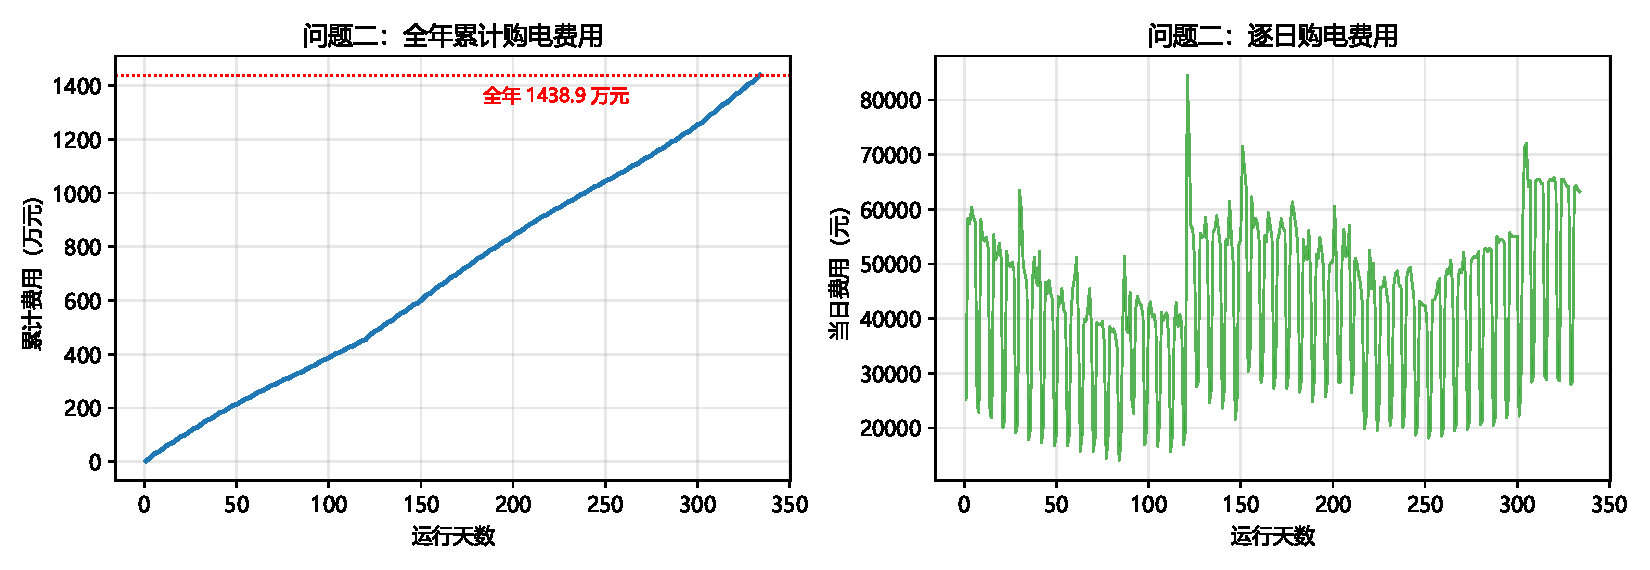
\includegraphics[width=0.85\textwidth]{q2_trend.pdf}
\caption{问题二全年费用的滚动累积曲线与预测方法对照}
\label{fig:q2-trend}
\end{figure}

% ==================== 五、问题三 ====================
\section{问题三：预报融合与场景树多时点调整}

\subsection{问题分析}

问题三在问题二基础上引入两项新要素：

\begin{enumerate}[itemsep=3pt,topsep=3pt]
  \item \textbf{多时点预报}：每天 $0$、$6$、$12$、$18$ 时各发布一次未来 24 h 的光伏整点预报，
        后续时刻的预报可用于\textbf{调整}购电策略；
  \item \textbf{调整计费}：调整不是免费的——
        计划量高于调整量的部分按 $50\%$ 违约电价、调整量高于计划量的部分按 $1.5$ 倍电价。
\end{enumerate}

因此模型需要回答两个层次的问题：
\textbf{(i) 如何在 0 点制定“预留调整余地”的计划：}
\textbf{(ii) 如何在后续发布时刻利用新信息最优地修正计划：}

\subsection{计费规则的统一化建模}
\label{sec:q3-fee}

设第 $t$ 段的 0 点原计划量为 $g_t^0$，最终调整后的购电量为 $q_t$。定义调增量与调减量

\begin{equation}
u_t=(q_t-g_t^0)_+,\qquad v_t=(g_t^0-q_t)_+,
\end{equation}

则 $q_t=g_t^0+u_t-v_t$。题面规则可统一写为

\begin{equation}
J=\sum_t\Bigl[\underbrace{p_tg_t^0}_{\text{原计划费}}
+\underbrace{1.5p_tu_t}_{\text{调增，1.5 倍}}
-\underbrace{p_tv_t}_{\text{退还原价}}
+\underbrace{0.5p_tv_t}_{\text{违约费，50\%}}
+\underbrace{5p_te_t}_{\text{紧急购电}}\Bigr].
\label{eq:q3-fee}
\end{equation}

即\textbf{净调整费为 $1.5p_tu_t-0.5p_tv_t$，它可以为负}。
合并同类项得另一便于独立核验的等价式：

\begin{equation}
J=\sum_t\Bigl[p_t\min(g_t^0,q_t)+0.5p_tv_t+1.5p_tu_t+5p_te_t\Bigr].
\label{eq:q3-fee2}
\end{equation}

\subsection{在线预报融合}

\subsubsection{融合权重}
\label{sec:q3-fusion}

设历史预测为 $H$、发布预报为 $F$、实际值为 $V$。只用最近 56 天内\textbf{已完全实现}的预报行，
以最小二乘拟合权重：

\begin{equation}
\alpha=\operatorname{clip}_{[0,1]}\frac{\sum(F-H)(V-H)}{\sum(F-H)^2},
\qquad \text{融合值}=\alpha F+(1-\alpha)H.
\label{eq:q3-alpha}
\end{equation}

\textbf{式 \eqref{eq:q3-alpha} 的推导}：以融合值与实际值的平方误差为目标
$\min_{\alpha}\sum\bigl[V-(\alpha F+(1-\alpha)H)\bigr]^2$。
记 $z=F-H$，则中括号内为 $(V-H)-\alpha z$，目标化为
$f(\alpha)=\sum\bigl[(V-H)-\alpha z\bigr]^2$。
对 $\alpha$ 求导并置零：
\begin{equation}
\frac{\mathrm{d}f}{\mathrm{d}\alpha}
=-2\sum z\bigl[(V-H)-\alpha z\bigr]=0
\ \Longrightarrow\ \alpha=\frac{\sum z\,(V-H)}{\sum z^2}.\label{eq:q3-alpha-deriv}
\end{equation}
又因二阶导 $\mathrm{d}^2f/\mathrm{d}\alpha^2=2\sum z^2>0$，
该驻点即全局极小点；再叠加 $[0,1]$ 截断以避免外推。
几何上，$\alpha$ 是 $V-H$ 在 $F-H$ 上的投影系数。

\textbf{收缩偏差校正}：进一步叠加历史平均残差的收缩估计
\begin{equation}
\text{偏差}=\overline{(V-\text{融合})}\cdot\frac{n}{n+14},
\end{equation}
其中 $n$ 为有效样本数。系数 $n/(n+14)$ 用于抑制小样本下偏差估计的波动：
样本充足时接近 $1$，样本稀少时被压缩向 $0$。

\subsubsection{发布预报的时间对齐}

附件 3 的“预报 $k$ 小时”是\textbf{发布时刻后第 $k$ 个整点}的\textbf{瞬时}功率，
而非第 $k$ 个小时区间的均值。故采用如下重建方式：

\begin{enumerate}[itemsep=2pt,topsep=3pt]
  \item 以 24 个整点为锚点，在 10 分钟网格上\textbf{线性插值}；
  \item 发布瞬间的端点使用\textbf{已观测}的实际光伏功率（0 点用前一日末观测值）。
\end{enumerate}

\noindent\textbf{为何不能把整点值当作“小时均值”：} 设真实光伏功率为正弦形的日间过程，
其峰谷差为 $A$、周期 $T_0=24$ h。若把第 $k$ 个整点的值 $v(k)$ 当作区间
$[k,k+1)$ 的均值作分段常数填充，相当于用左端点值代替中点值，
引入的按时段均值计的系统偏差为
\begin{equation}
\overline{\varepsilon}=\frac{1}{T_0}\int_0^{T_0}\bigl[v(k)-v(t)\bigr]\,\mathrm{d}t\ \sim\ \frac{1}{2}\cdot\frac{\mathrm{d}v}{\mathrm{d}t}\cdot 1\ \text{h},
\label{eq:q3-phase}
\end{equation}
即在梯度最大处（日出、日落）偏差最大，量级为\textbf{半小时}的光伏变化量，
故称 “$1/2$ 小时量级的系统相位误差”。线性插值则以相邻两整点为端点，
把该项偏差从 $O(\Delta)$ 降到 $O(\Delta^2)$，且在每个整点上无偏。

\noindent\textbf{实证核对：} 以附件 2 的实际光伏为基准，用两种方式重建同一预报行的
144 段并逐段比较（除去最后一天以避开跨年缺口），结果见表 \ref{tab:q3-align}。

\begin{table}[H]
\centering
\caption{两种整点重建方式的全年逐段 MAE（kW，365 天平均）}
\label{tab:q3-align}
\begin{tabular}{@{}l r r r@{}}
\toprule
发布时间 & 分段常数填充 & \textbf{线性插值（本文）} & 降幅 \\
\midrule
$0$ 点  & 440.64 & \textbf{225.99} & $-48.7\%$ \\
$6$ 点  & 405.15 & \textbf{167.39} & $-58.7\%$ \\
$12$ 点 & 453.61 & \textbf{238.10} & $-47.5\%$ \\
$18$ 点 & 488.43 & \textbf{292.97} & $-40.0\%$ \\
\bottomrule
\end{tabular}
\end{table}

\noindent 线性插值在四个发布时间上把逐段 MAE 降低 $40.0\%$--$58.7\%$，
与式 \eqref{eq:q3-phase} 的机理一致：分段常数填充在日出、日落的高梯度处偏差最大，
而线性插值恰在这些位置把误差从 $O(\Delta)$ 降到 $O(\Delta^2)$。
这说明\textbf{时间对齐方式本身是预报误差的一个可测量来源}，而非实现细节。
需要说明的是，表 \ref{tab:q3-align} 度量的是“给定整点预报下的重建误差”，
而图 \ref{fig:q3-fusion} 展示的是融合后的综合预报精度，两者口径不同、不可直接相减。

\subsection{经验场景树}

\subsubsection{信息限制：非前视约束（本问的建模前提）}
\label{sec:q3-nonanticip}

问题二已要求“预测只能用历史数据”，
本问把它\textbf{进一步强化}到“场景树的节点划分也只能依据届时已发布的信息”，
原因是本问新增了多个决策时点，若不限制就可能在 6 点“提前知道” 12 点才会发布的信息。
具体为三条：
\begin{itemize}[itemsep=2pt,topsep=3pt]
  \item 训练样本仅取\textbf{不晚于 $d-2$ 天发布}的预报行，
        以确保跨午夜的未来 24 h 已经实现；
  \item 每个发布时刻\textbf{分别}训练，不得利用当天后续发布的预报来估计当前权重；
  \item 样本少于 7 条时退化为直接使用发布预报。
\end{itemize}

\noindent 上述约束在模型中的实现方式是“节点内共享变量”，
见 \S\ref{sec:q3-tree}；它比额外添加约束更稳健，因为物理上不可能针对已知场景分别决策。

\subsubsection{场景构造}

在第 $a$ 次发布时刻，场景净负载为

\begin{equation}
N_{s,t}=\hat N_t^{(a)}+\Bigl(N_{r_s,t}-\hat N_{r_s,t}^{(a)}\Bigr),
\label{eq:q3-scen}
\end{equation}

即用历史日 $r_s$ 在\textbf{同一发布时刻}的残差去修正当前的发布预报。

\subsubsection{信息分支（场景树）}
\label{sec:q3-tree}

仅用点预测场景会丢失一个重要信息：\textbf{不同历史日不仅能告诉我们“缺口可能多大”，
还能告诉我们“预报会如何变化”}。为此把场景组织为树：

\begin{enumerate}[itemsep=3pt,topsep=3pt]
  \item 历史日 $r_s$ 除净负载残差外，还附带它在\textbf{后续发布时刻}的预报修订向量；
  \item 把这些修订作为“未来可能观测到的信息”，用\textbf{二叉聚类}（按方差最大的维度二分）
        组织成树；
  \item \textbf{关键的非前视要求}：每个节点只能依据\textbf{届时新发布的预报修订}划分其子节点，
        不得使用尚未实现的未来负载或实际光伏；
  \item 节点概率 $\pi_n=$ 落入该节点的历史日数 $/$ 总样本数；
  \item 树最多 4 层、15 个决策节点；\textbf{全部 56 条残差样本仍参与期望缺口成本}，
        未把场景简化为少数均值曲线。
\end{enumerate}

\begin{figure}[H]
\centering
\begin{tikzpicture}[scale=1.0,every node/.style={font=\small},
   nd/.style={circle,draw,fill=blue!8,minimum size=6.5mm,inner sep=0pt},
   lf/.style={rectangle,draw,fill=green!10,minimum size=5mm,inner sep=2pt}]
  \node[nd] (r) at (0,0) {$0$};
  \node[nd] (a) at (2.2,1.3) {$1$};
  \node[nd] (b) at (2.2,-1.3) {$2$};
  \node[nd] (c) at (4.6,2.0) {$3$};
  \node[nd] (d) at (4.6,0.7) {$4$};
  \node[lf] (e) at (6.9,1.4) {$\vdots$};
  \node[lf] (f) at (6.9,-0.4) {$\vdots$};
  \draw (r)--(a) node[midway,above,sloped,font=\scriptsize]{$6$ 时修订};
  \draw (r)--(b);
  \draw (a)--(c) node[midway,above,sloped,font=\scriptsize]{$12$ 时修订};
  \draw (a)--(d);
  \draw (c)--(e) node[midway,above,sloped,font=\scriptsize]{$18$ 时};
  \draw (d)--(f);
  \node[font=\scriptsize,align=left] at (0,-2.3)
    {节点内\textbf{共享} $q,c,d,E$；\\ 仅 $e_{s,t}$ 按场景不同};
\end{tikzpicture}
\caption{经验场景树结构（示意）：顺着“新发布的预报修订”逐层分支，节点内共享控制变量}
\label{fig:q3-tree}
\end{figure}

\vspace{0.2em}
\noindent\textbf{为何“节点内共享变量”能保证非前视：}
因为控制变量 $q,c,d,E$ 是\textbf{同一个变量}跨越该节点内的所有场景，
物理上不可能针对“已经知道是哪个场景”来分别决策——
这在变量结构层面（而非仅通过额外约束）排除了前视。

\subsection{场景树随机规划模型}

以节点 $n$ 为单位，其概率为 $\pi_n$，控制变量为 $q_{n,t},c_{n,t},d_{n,t},E_{n,t}$：

\begin{equation}
\min\ J_3=\sum_tp_tg_t^0
+\sum_n\pi_n\sum_{t\in n}\bigl(1.5p_tu_{n,t}-0.5p_tv_{n,t}\bigr)
+\frac{1}{S}\sum_s\sum_t5p_te_{s,t}
+\underbrace{\text{次日前瞻成本}}_{\text{价值近似}}.
\label{eq:q3-obj}
\end{equation}

约束：

\begin{align}
&\text{（调整关系）}\quad q_{n,t}=g_t^0+u_{n,t}-v_{n,t},\qquad q,u,v\ge 0, \label{eq:q3-adj}\\
&\text{（节点需求）}\quad q_{n,t}+d_{n,t}-c_{n,t}+e_{s,t}\ \ge\ N_{s,t},\qquad e_{s,t}\ge0, \label{eq:q3-dem}\\
&\text{（计划下界）}\quad q_{n,t}+d_{n,t}-c_{n,t}\ \ge\ \hat N_t, \label{eq:q3-floor}\\
&\text{（SOC 与容量）}\quad E_{n,t}=E_{n,t-1}+0.9c_{n,t}-\frac{d_{n,t}}{0.9},\quad
   1200\le E_{n,t}\le10800, \label{eq:q3-soc}\\
&\text{（功率）}\quad 0\le c_{n,t},d_{n,t}\le\frac{5000}{6}, \label{eq:q3-pow}\\
&\text{（父子衔接）}\quad E_{n,\text{首}}=E_{\text{父},\text{末}}. \label{eq:q3-link}
\end{align}

\subsection{跨日价值与贪心执行}

\textbf{跨日前瞻}：每次优化至\textbf{次日 24 点}，把次日作为确定性价值近似，
避免“只顾当天便宜电价而提前耗空电池”。
不同未来节点使用其条件预报修订后的次日点预测。

\textbf{贪心执行}：只执行当前发布到下一允许更新前的控制量：

\begin{center}
\begin{tabular}{@{}c c@{}}
\toprule
决策时刻 & 本次执行区间 \\
\midrule
$0$:00  & $0$--$6$ 时 \\
$6$:00  & $6$--$12$ 时 \\
$12$:00 & $12$--$18$ 时 \\
$18$:00 & $18$--$24$ 时 \\
\bottomrule
\end{tabular}
\end{center}

\noindent\textbf{为何不把问题二的 $80\%$ 分位直接套用到本问：}
问题二的 $F^*=0.80$ 是在“储能固定、单期补救费为 $5$ 倍、无后续调整”
条件下导出的单期临界分位；而问题三中 0 点可从场景树\textbf{评估未来的调整机会}，
今天的“少买”可在 6/12/18 点以 $1.5$ 倍价补上，故有效风险水平随节点、时段而变，
不应硬编码单一分位。这正是不用报童模型而用场景树多阶段模型的原因。
（同时充放电的处理与问题一相同：由 \S\ref{sec:q1-tight} 的等 SOC 扰动自动消去，
程序对最终执行结果逐段检查互斥。）

\subsection{结果与边际分析}

\begin{table}[H]
\centering
\caption{问题三：更新频率对照与逐级边际收益（2 月 1 日--12 月 31 日）}
\label{tab:q3-abl}
\begin{tabular}{@{}l r r l@{}} 
\toprule
方案 & {总费用（元）} & {紧急电量（kWh）} & {增量节省（元）} \\
\midrule
方案 B 框架同口径复算 & 14389892.50 & 246099.33 & — \\
仅 0 点融合预报       & 14181445.03 & 218589.30 & 208447.47 \\
$0$、$6$ 点           & 14101371.47 & 186570.89 & 80073.56 \\
$0$、$6$、$12$ 点     & 14022358.10 & 175344.39 & 79013.36 \\
\textbf{$0$、$6$、$12$、$18$ 点（主方案）} & \bfseries 14022396.98 & 175369.95 & $-38.88$ \\
\bottomrule
\end{tabular}
\end{table}

\begin{table}[H]
\centering
\caption{问题三主方案费用分解}
\label{tab:q3-fee}
\begin{tabular}{@{}l r@{}}
\toprule
项目 & {金额（元）} \\
\midrule
原计划购电费      & 13345819.30 \\
增购费（$1.5$ 倍）  & 89947.28 \\
取消原费退款      & $-150170.13$ \\
取消违约费（$50\%$）& 75085.07 \\
净调整费（小计）    & 14862.22 \\
紧急购电费（$5$ 倍）& 661715.46 \\
\midrule
\textbf{总费用} & \bfseries 14022396.98 \\
\bottomrule
\end{tabular}
\end{table}

相对同口径方案 B，主方案\textbf{节省 $367\,495.52$ 元（$2.55\%$）}，
紧急购电量\textbf{减少 $28.74\%$}。
\textbf{结论}：$6$ 点与 $12$ 点各贡献约 $8$ 万元，收益随调整次数\textbf{显著边际递减}；
$18$ 点更新在本年度回测中\textbf{无可观测收益}（$-38.88$ 元），可视为可选更新。
该结论限于本数据与算法：$18$ 点仍可能通过次日预报影响跨日储能，
且小型经验树在有限样本下重建，不保证费用随信息增加单调下降。

\begin{figure}[htbp]
\centering
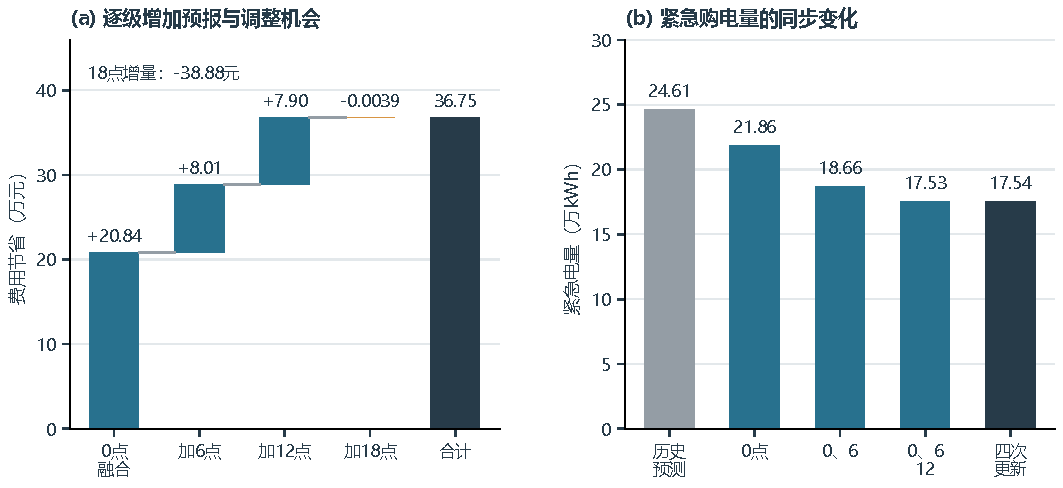
\includegraphics[width=0.88\textwidth]{04_q3_information_value.pdf}
\caption{固定电价情形下的逐级费用节省与紧急购电量。费用节省以本问同口径
历史预测对照为起点，依次引入 0 点融合预报和 6、12、18 点调整；
右图按相同顺序比较紧急购电量。}
\label{fig:q3-info-value}
\end{figure}

图 \ref{fig:q3-info-value} 把“信息更新的价值”与“更新次数的增加”分开呈现：
仅引入 0 点融合预报即节省 $208\,447.47$ 元；
随后增加 6 点与 12 点更新各节省约 $8$ 万元；增加 18 点后费用反而上升 $38.88$ 元。
这说明\textbf{预报融合本身的价值最大，而更新次数存在明显边际递减}。

\begin{figure}[htbp]
\centering
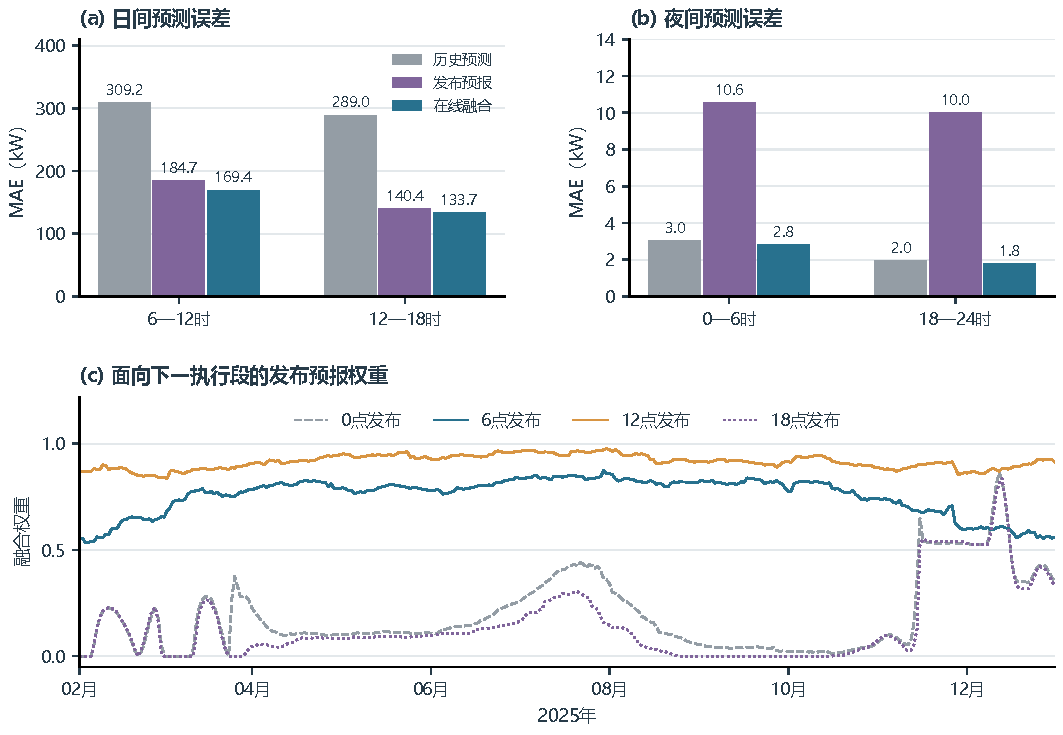
\includegraphics[width=0.88\textwidth]{05_q3_forecast_fusion.pdf}
\caption{发布后六小时光伏预测误差及融合权重。(a)(b) 分别比较日间和夜间的
历史预测、发布预报及在线融合 MAE，两面板纵轴尺度不同；
(c) 展示各发布时间对应的发布预报权重。}
\label{fig:q3-fusion}
\end{figure}

6--12 时段的 MAE 由历史预测的 $309.24$ kW 降至融合预测的 $169.41$ kW，
12--18 时段由 $288.99$ kW 降至 $133.68$ kW。夜间绝对误差较小，单独绘制以保留其变化尺度。
融合权重随历史已成熟样本更新，并包含偏差校正，因此融合输出不只是当期两条预报的
固定加权平均。\textbf{MAE 改善本身不等同于等比例的费用下降}，
经济效果须结合图 \ref{fig:q3-info-value} 的更新频率对照判断。

\begin{figure}[htbp]
\centering
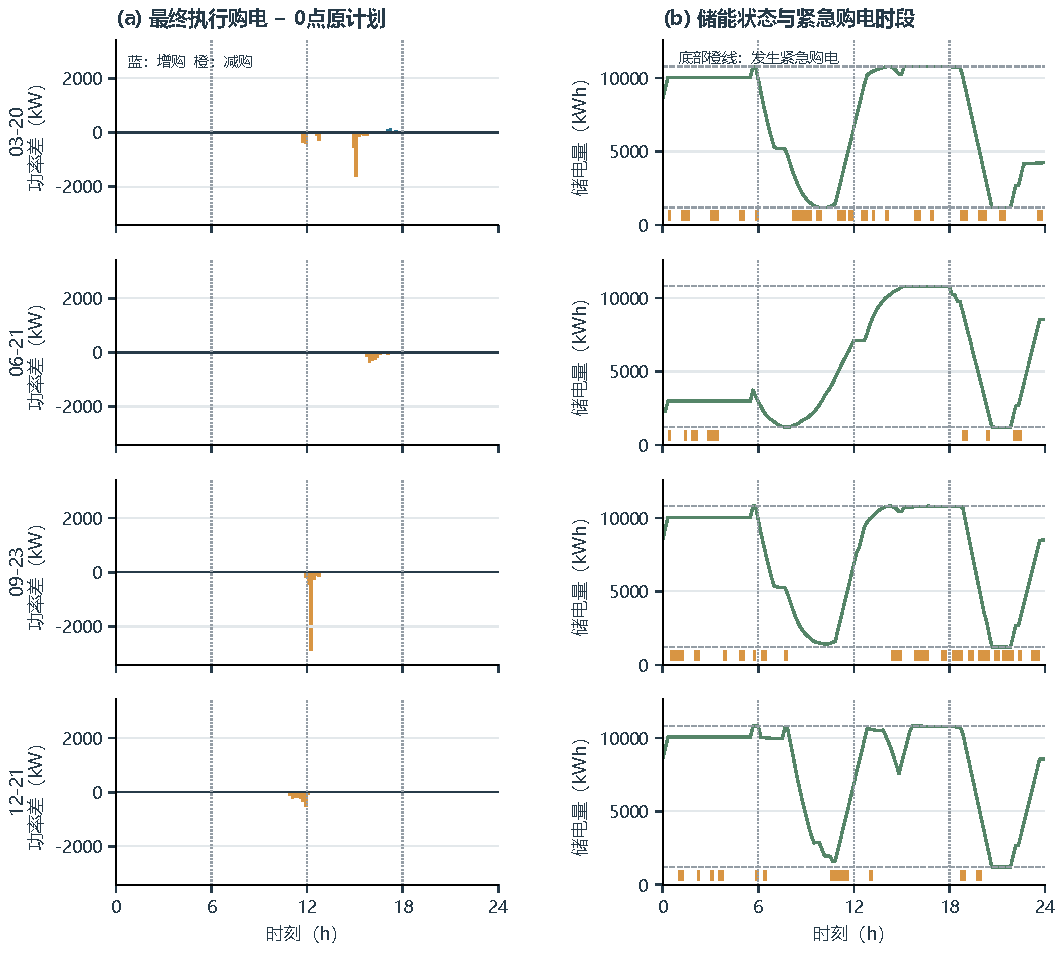
\includegraphics[width=0.88\textwidth]{06_q3_rolling_adjustment.pdf}
\caption{四个指定日的日内计划修正与储能状态。左列为最终执行购电相对 0 点原计划的
功率差，正值为增购、负值为减购；右列为储电量，底部橙色短线标记紧急购电
大于数值容差的时段。竖虚线表示 6、12、18 点发布时刻。}
\label{fig:q3-adjust}
\end{figure}

日内更新后的购电修正相对原计划较小，直接叠加两条绝对购电曲线容易掩盖变化；
以原计划为零基准后，可清楚识别各执行区间内的增购与减购。
储电量按跨日滚动过程衔接，指定日的首末电量不要求逐日相等。
紧急购电标记只表示发生时间，不表示缺口大小，
也不能据其与储能状态的相邻关系断言单一原因。

\FloatBarrier

\subsection{敏感性分析与性能边界}
\label{sec:q3-sens}

\textbf{完美预见下界}：假设每天 $0$ 点即精确知道当天实际净负载（消除全部预报误差），
在同一物理约束与计费规则下求解得下界 $1\,223.16$ 万元（紧急购电费为 $0$），
与主方案 $1\,402.24$ 万元相差 $179.08$ 万元——\textbf{该缺口全部来自预报误差，而非建模策略}。

\textbf{融合权重的饱和性}：逐日自适应融合的加权 MAE 为 93.68 kW，
\textbf{优于含未来信息泄漏的静态最优线性组合}（95.08 kW），
说明权重估计已实质达到该模型族的精度上界。

\textbf{参数扫描（30 余组）}：对场景缩放、残差窗口、收缩参数、计划下界、多源信息等
做同年度扫描，仅“场景缩放 $k=0.92$”有正收益（约 $0.47$ 万元，$0.03\%$），
其余全部无效或变差（窗口 $W=28$ 时 $+5.31$ 万元、计划下界 $0.5\times$ 时 $+12.15$ 万元）。
未把 $k=0.92$ 写入正式结果——同年度扫描存在过拟合风险，收益量级可忽略。

\textbf{注意到}：（1）\textbf{弃置电量并非浪费}——全年弃置 $267.66$ 万 kWh，
但放松计划下界反而使总费用上升，原因是“多买的电”是“低价购电 $+$ 储能套利”的必要冗余；
（2）\textbf{增加信息源可能有害}——“上一期发布”虽合法可用，但纳入融合后费用上升
$+0.66$ 万元，因多次发布高度相关，额外信息源主要引入估计噪声。

\noindent\textbf{结论的适用范围}：以上只能说明“在已测试模型族与同年度回测下未发现更优”，
\textbf{不足以宣称全局最优}；引入外部气象数据仍有提升余地。

% ==================== 六、问题四 ====================
\section{问题四：实时波动电价下的调度}

\subsection{问题分析与总体思路}

问题四指出外网电价也是\textbf{实时波动}的，要求在此条件下重算问题二（记为 4-2）
与问题三（记为 4-3）。与前三问的关系如下：

\begin{center}
\begin{tabular}{@{}l l l@{}}
\toprule
 & 电价 & 决策时点 \\
\midrule
问题二  & 每日固定（附件 1）    & 仅 $0$:00 \\
\textbf{4-2} & \textbf{实时波动（附件 4）} & 仅 $0$:00 \\
问题三  & 每日固定              & $0/6/12/18$ 时 \\
\textbf{4-3} & \textbf{实时波动}      & $0/6/12/18$ 时 \\
\bottomrule
\end{tabular}
\end{center}

因此 4-2 是“问题二 $+$ 电价随机性”，4-3 是“问题三 $+$ 电价随机性”。
两问均需解决一个新问题：\textbf{电价本身也未知，如何构造决策所需的场景？}

\subsection{4-2：波动电价下的日前调度}

\subsubsection{电价信息的假设（本问的关键判断）}

题面说明电价实时波动，但\textbf{未明确每天 $0$:00 是否已知全天价格}。
这个信息假设对结果影响很大，故我们保留两种情形并\textbf{分别完整求解}：

\begin{table}[H]
\centering
\caption{4-2 的两种电价信息情形}
\begin{tabular}{@{}l l l@{}}
\toprule
情形 & 假设 & 性质 \\
\midrule
\textbf{主模型} & 当天电价\textbf{未知}，只用此前日期预测 & 保守、符合“实时波动”的通常理解 \\
对照         & 当天 144 段电价已于 $0$:00 公布 & 明确放宽信息限制 \\
\bottomrule
\end{tabular}
\end{table}

主模型不把当天或未来的实际电价、负载、光伏作为制定当天计划的输入；
附件 4 的实际电价仅用于\textbf{事后结算}。

\subsubsection{电价预测器选择}

只用 1 月 8--31 日的 24 个历史预测日，比较四种规则：

\begin{enumerate}[itemsep=2pt,topsep=3pt]
  \item 前一日曲线；
  \item 近 7 日均值；
  \item 近 7 日形状 $+$ 前一日平均水平；
  \item 最近 4 次同星期几均值。
\end{enumerate}

以 1 月预测的 RMSE 选定，\textbf{2 月起固定方法不再更换}，避免用全年费用反向挑选参数。
入选方法为\textbf{最近 4 次同星期几均值}：

\begin{equation}
\hat p_{d,t}=\frac{1}{|\mathcal W_d|}\sum_{i\in\mathcal W_d}p_{i,t},
\qquad \mathcal W_d=\{d-7j:\ j=1,\dots,4,\ d-7j\ge0\}.
\end{equation}

预测 $d+1$ 日时进一步要求所有样本日期 $i<d$，不得使用尚未发生的第 $d$ 日价格。

\subsubsection{电价—净负载联合场景}

\textbf{核心论证：期望的不可分解性。}
当电价随机时，
\begin{equation}
\E\bigl[p_t(N_t-z_t)_+\bigr]\ \neq\ \E[p_t]\cdot\E\bigl[(N_t-z_t)_+\bigr].
\label{eq:q4-nonsep}
\end{equation}
不等式成立的原因是：\textbf{高电价可能与缺电同时发生}
（例如极端天气既推高需求又推高价格）。
若按式 \eqref{eq:q4-nonsep} 右端建模（即“平均电价近似”），
会系统性地\textbf{低估}缺电风险的实际代价。

因此场景\textbf{取自同一历史日}的两种残差配对：

\begin{equation}
N_{s,t}=\hat N_{d,t}+r^N_{s,t},\qquad
p_{s,t}=\max\bigl\{0.001,\ \hat p_{d,t}+r^p_{s,t}\bigr\},
\label{eq:q4-scen}
\end{equation}

其中 $r^N_{s,t}=N_{s,t}-\hat N_{s,t}$、$r^p_{s,t}=p_{s,t}-\hat p_{s,t}$ 均由历史日 $s$ 产生。
$0.001$ 元/kWh 是预先给定的正数下限，用于防止加性误差生成负电价，
被截断的场景数逐日记录以便审查。

场景集为 $\mathcal H_d=\{\max(7,d-56),\dots,d-1\}$，等权 $\omega_s=1/|\mathcal H_d|$。

\subsubsection{目标函数}

当天计划 $g,c,d$ 在所有场景间共享，紧急购电 $u_{s,t}$ 可随场景变化：

\begin{equation}
\min\ J_{42}=\sum_{t=1}^{144}\overline p_{d,t}\,g_t
+5\sum_s\omega_s\sum_{t=1}^{144}p_{s,t}\,u_{s,t}
+\underbrace{\sum_{t=1}^{144}\hat p_{d+1|d,t}\,g_{144+t}}_{\text{次日前瞻价值（不进报表）}},
\label{eq:q4-obj}
\end{equation}

其中 $\overline p_{d,t}=\sum_s\omega_s p_{s,t}$ 为场景平均电价，用于第一阶段购电费（计划量照付）。

\textbf{风险覆盖的分位解释}：固定某段的 $c,d$，令 $z=g+d-c$，
则其覆盖水平可用\textbf{电价加权分位}理解
\begin{equation}
\widetilde\omega_{s,t}=\frac{\omega_s p_{s,t}}{\overline p_{d,t}},\qquad
z\approx Q^{\widetilde\omega}_{0.8}(N_{s,t}),
\end{equation}
即高电价的场景会获得更高权重，从而抬高所需的供给水平。
但该式只是启发式解释，实际须与储能跨时段约束一并求解，不能逐段套用。

\subsubsection{约束与对照模型}

约束沿用问题二：计划下界 \eqref{eq:q2-floor}、场景兜底 \eqref{eq:q2-scen}、
SOC 与容量功率 \eqref{eq:q2-soc}--\eqref{eq:q2-cap}，以及 48 h 窗口终端条件。
另外设置\textbf{平均电价对照}：保留完全相同的净负载场景，
但把所有 $p_{s,t}$ 替换为 $\overline p_{d,t}$，以检验“配对关系”的实际作用。

\subsubsection{结果}

\begin{table}[H]
\centering
\caption{4-2 结果对照（2 月 1 日--12 月 31 日）}
\label{tab:q42}
\begin{tabular}{@{}l r r r@{}}
\toprule
方案 & {总费用（元）} & {较 Q2 重结算（元）} & {节省比例} \\
\midrule
原 Q2 计划按附件 4 重结算 & 15184704.23 & — & — \\
平均电价模型              & 15160921.45 & $-23782.79$ & $0.157\%$ \\
\textbf{联合场景模型（主）} & \bfseries 15163043.89 & \bfseries $-21660.34$ & $0.143\%$ \\
当日电价已知（对照）       & 15033043.18 & $-151661.05$ & $0.999\%$ \\
\bottomrule
\end{tabular}
\end{table}

\textbf{诚实说明}：在同年回测中，平均电价近似\textbf{略优于}联合场景
（差约 $2\,122$ 元）。我们不因此改用平均电价模型，理由有二：
(i) 联合场景保留了正确的概率结构（式 \eqref{eq:q4-nonsep} 说明它的期望是准确的），
(ii) 单一年度的 $2\,122$ 元差异不具统计显著性，而结构性正确性可跨年成立。
这一现象在结果文件中如实保留。

\textbf{“当日电价已知”的增益}：$151\,661.05$ 元（约 $1.0\%$），
说明\textbf{电价预测误差}是本问剩余成本的主要来源之一。

\begin{figure}[htbp]
\centering
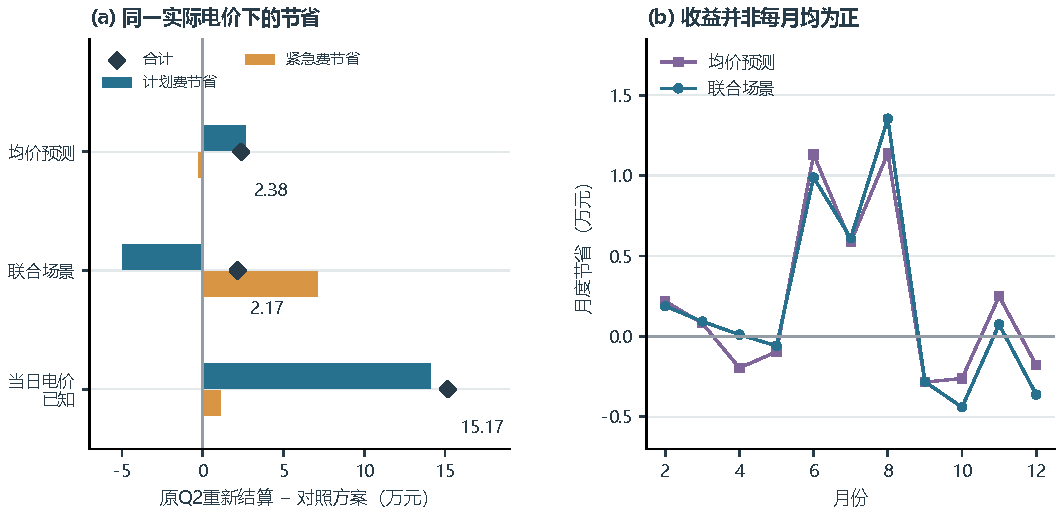
\includegraphics[width=0.95\textwidth]{07_q42_price_information.pdf}
\caption{相对原第二问策略按附件 4 电价重新结算的费用节省。左图将节省分为
计划费与紧急费，菱形表示合计，负值表示该项费用增加；
右图展示均价预测与联合场景的月度净节省。当日电价已知为信息对照。}
\label{fig:q42-info}
\end{figure}

图 \ref{fig:q42-info} 显示月度节省存在正负变化：年度改善不保证各月均改善，
且均价预测方案在本年度略优（见上文说明）。该图同时说明
“信息更充分”与“当月费用更低”不总是同步。

\begin{figure}[htbp]
\centering
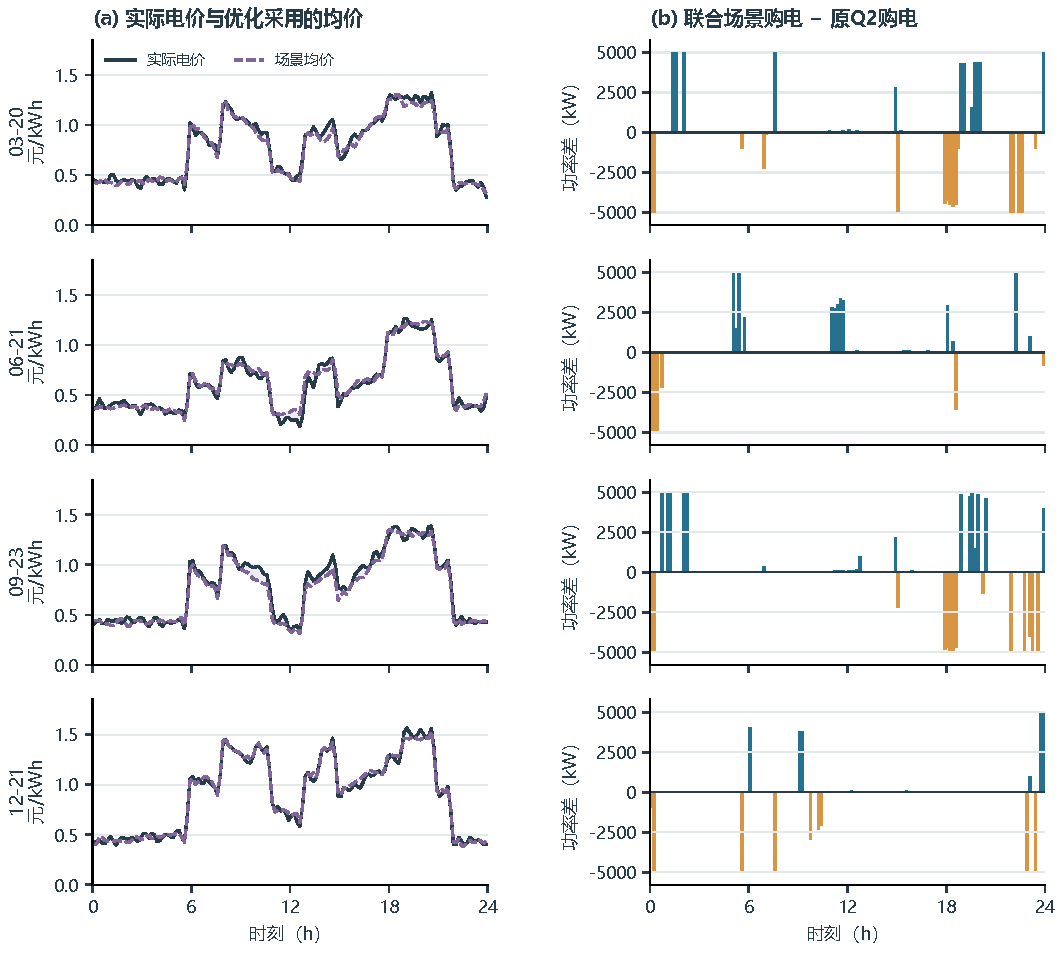
\includegraphics[width=0.95\textwidth]{08_q42_schedule_shift.pdf}
\caption{四个指定日的实际电价、优化采用的场景均价及购电计划差异。
左列阴影仅表示两条价格曲线的差距；右列为联合场景计划购电功率
减去原 Q2 计划购电功率，蓝色为增购、橙色为少购。}
\label{fig:q42-shift}
\end{figure}

将原第二问策略作为参照，可以观察到价格信息模型引入后购电时段发生重排。
场景均价与实际电价并不处处一致，价格曲线形状接近也不保证决策完全相同。
联合场景的决策还依赖价格与净负载误差的配对、储能约束及前期形成的状态，
因此左、右两列用于对照现象，不将每个购电差值单独归因于同一时段的价格预测误差。
此处展示的是日前计划，不应描述为当天观察实际价格后的日内修正。

\begin{figure}[H]
\centering
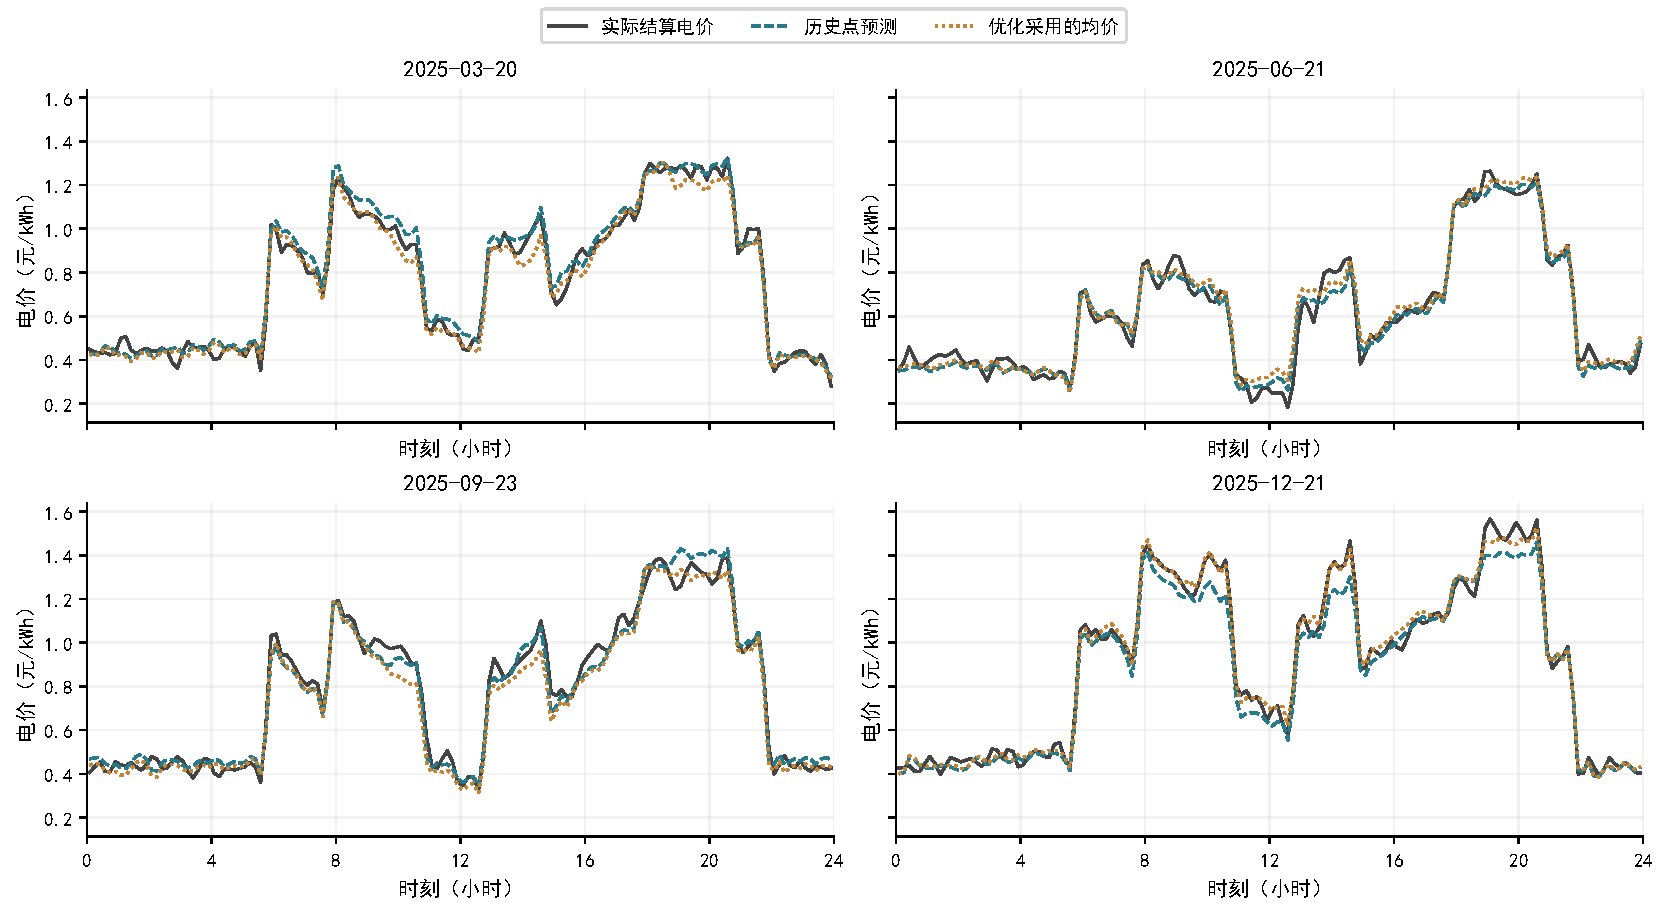
\includegraphics[width=0.9\textwidth]{q42_prices.pdf}
\caption{4-2：指定日期的实际电价曲线与预测电价}
\label{fig:q42-prices}
\end{figure}

\begin{figure}[H]
\centering
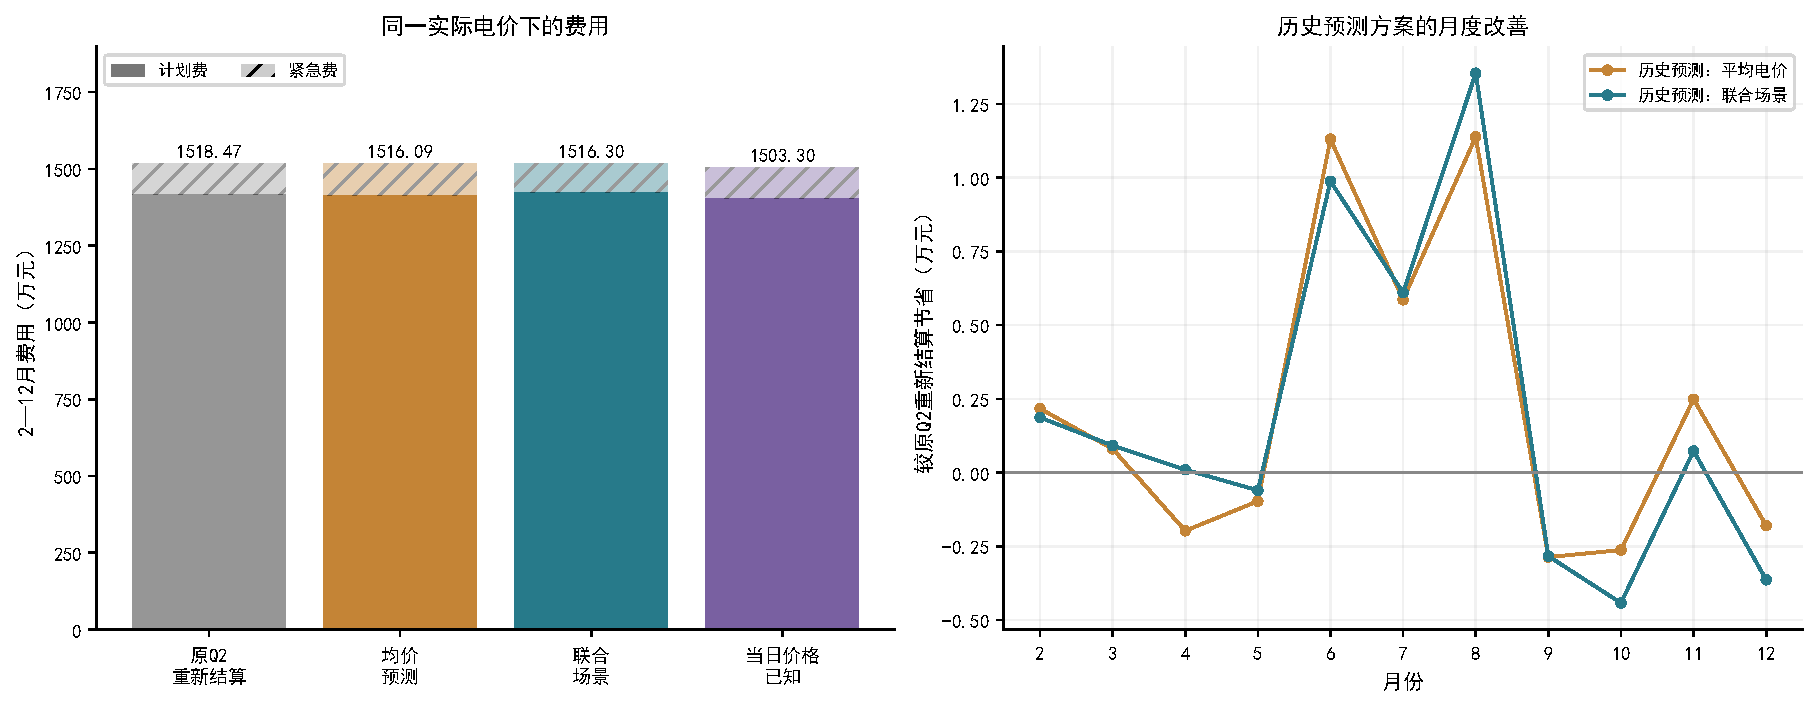
\includegraphics[width=0.9\textwidth]{q42_cost.pdf}
\caption{4-2：各方案费用对照}
\label{fig:q42-cost}
\end{figure}

\FloatBarrier

\subsection{4-3：波动电价 $+$ 多时点调整}

\subsubsection{模型构造}

4-3 在 4-2 的基础上叠加问题三的多时点调整机制：每天 $0$ 点定计划，
$6/12/18$ 点用新发布的光伏预报与更新的电价预测重新优化尚未执行的调度。
计费规则（调增 $1.5$ 倍、调减净成本 $-0.5$ 倍、紧急 $5$ 倍）与问题三完全一致，
即沿用式 \eqref{eq:q3-fee}。

\textbf{电价场景的处理}：每次发布时刻对未来电价采用
\textbf{此前 7 天同一时段均值}，并与同一历史日的净负载残差\textbf{配对}构造价格场景
（保留式 \eqref{eq:q4-scen} 的相关性结构）。次日采用历史价格预测。

\textbf{场景树、融合与执行}：与问题三相同——使用经验场景树保证非前视，
用在线融合整合历史预测与发布预报，只执行当前发布到下一更新前的控制量。

\subsubsection{结果}

\begin{table}[H]
\centering
\caption{4-3 主方案费用分解}
\label{tab:q43}
\begin{tabular}{@{}l r@{}}
\toprule
项目 & {金额（元）} \\
\midrule
原计划购电费       & 13457230.68 \\
增购费（$1.5$ 倍）   & 152250.38 \\
取消原费退款       & $-173200.59$ \\
取消违约费（$50\%$） & 86600.30 \\
净调整费（小计）     & 65650.08 \\
紧急购电费（$5$ 倍） & 1538854.67 \\
\midrule
\textbf{总费用} & \bfseries 15061735.43 \\
\bottomrule
\end{tabular}
\end{table}

\subsubsection{关键对比：调整机制价值的同口径分解}

固定电价（问题三）与波动电价（4-3）两问都建立了\emph{逐级增量}的对照方案，
故可对两问做\textbf{口径完全对称}的分解。下表左半为各方案总费用（元），
右半为由此得到的收益分解（万元）：

\begin{table}[H]
\centering
\small
\caption{两问逐级增量对照与同口径分解（结果期均 334 天）}
\label{tab:q4-compare}
\setlength{\tabcolsep}{4pt}
\begin{tabular}{@{}l r r@{\hskip 8pt}l r r@{}}
\toprule
方案 & 固定电价 & 波动电价 & 收益来源 & 固定 & 波动 \\
\midrule
无融合，仅 $0$ 点（B）    & 14389892.50 & 15516984.54
  & ① 在线预报融合 & $20.84$ & $22.19$ \\
融合预报，仅 $0$ 点       & 14181445.03 & 15295120.10
  & ② 多时点调整 & $15.90$ & \bfseries $23.34$ \\
融合 $+$ $0/6$ 点         & 14101371.47 & 15173094.46
  & \quad 加 $6$ 点  & $8.01$ & $12.20$ \\
融合 $+$ $0/6/12$ 点      & 14022358.10 & 15068610.47
  & \quad 加 $12$ 点 & $7.90$ & $10.45$ \\
\textbf{融合 $+$ $0/6/12/18$ 点} & \bfseries 14022396.98 & \bfseries 15061735.43
  & \quad 加 $18$ 点 & $-0.004$ & $+0.69$ \\
\bottomrule
\end{tabular}
\end{table}

“无融合 B 方案 $\to$ 主方案”的总改善可拆成\textbf{融合预报}与\textbf{多时点调整}
两部分，两者之和恒等于总改善（固定电价 $36.75$ 万、波动电价 $45.52$ 万）。
可见\textbf{在完全同口径下，波动电价显著放大了多时点调整的价值}：
由 $15.90$ 万元增至 $23.34$ 万元（\textbf{高约 $47\%$}），
而融合预报的价值仅由 $20.84$ 万元增至 $22.19$ 万元（高约 $7\%$）。
调整机制的相对重要性由 $43\%$（$15.90/36.75$）提升到 $51\%$（$23.34/45.52$），
\emph{超过了融合预报}。

这一点还可从\textbf{边际递减形态}上看出差异：固定电价下第三次调整
（加 $18$ 点）已经\textbf{零收益}（$-38.88$ 元），
而波动电价下仍有 $+6\,875$ 元正收益——说明电价波动\emph{推迟了}调整机制的饱和点。
原因在于电价波动引入了\textbf{第二个不确定性来源}：多时点更新不仅能修正光伏预报，
还能修正\textbf{电价预期}，当新信息显示“傍晚电价将冲高”时，
可及时调整购电与储能部署，这是固定电价下不存在的收益渠道。

需要强调：$4\text{-}2 \to 4\text{-}3$ 的\textbf{主方案}差值为 $101\,308.46$ 元，
但该差值横跨两问，同时包含“预测源切换”与“引入调整机制”两种效应，
\textbf{不能}作为调整机制的边际价值；上表的逐级增量才是同口径度量。
两问主方案的绝对费用仍相差约 $104$ 万元，主要来自附件 4 的实时电价整体高于附件 1。

\begin{figure}[htbp]
\centering
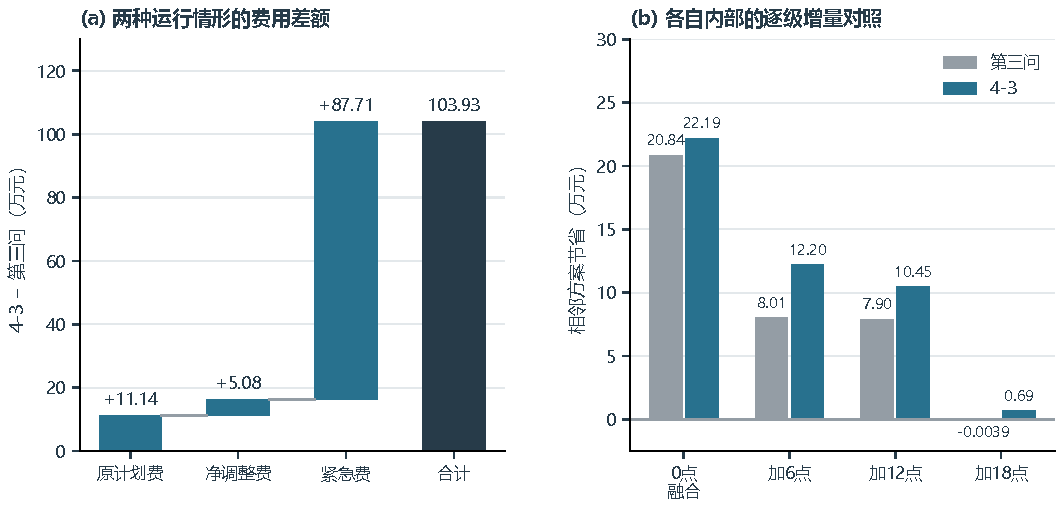
\includegraphics[width=0.95\textwidth]{09_q43_incremental_comparison.pdf}
\caption{4-3 与第三问主方案的费用差额及更新收益比较。左图按原计划费、
净调整费和紧急费分解 4-3 减第三问的总费用差；右图分别在两问内部
计算相邻更新方案之间的费用节省。}
\label{fig:q43-incremental}
\end{figure}

4-3 主方案费用为 $15\,061\,735.43$ 元，比第三问高 $1\,039\,338.45$ 元，
其中紧急费差额为 $877\,139.21$ 元，占总差额的 $84.39\%$。
该结果是不同电价输入及对应滚动策略共同形成的账面差异，
不能全部解释为电价波动或预测误差的因果成本。在各自内部的逐级对照中，
增加 6 点更新的节省由第三问的 $8.01$ 万元变为 4-3 的 $12.20$ 万元，
增加 12 点由 $7.90$ 万元变为 $10.45$ 万元；4-3 增加 18 点节省 $6\,875.04$ 元，
而第三问费用增加 $38.88$ 元。这表明新增调整机会的回测价值随运行情形而变化。

\begin{figure}[htbp]
\centering
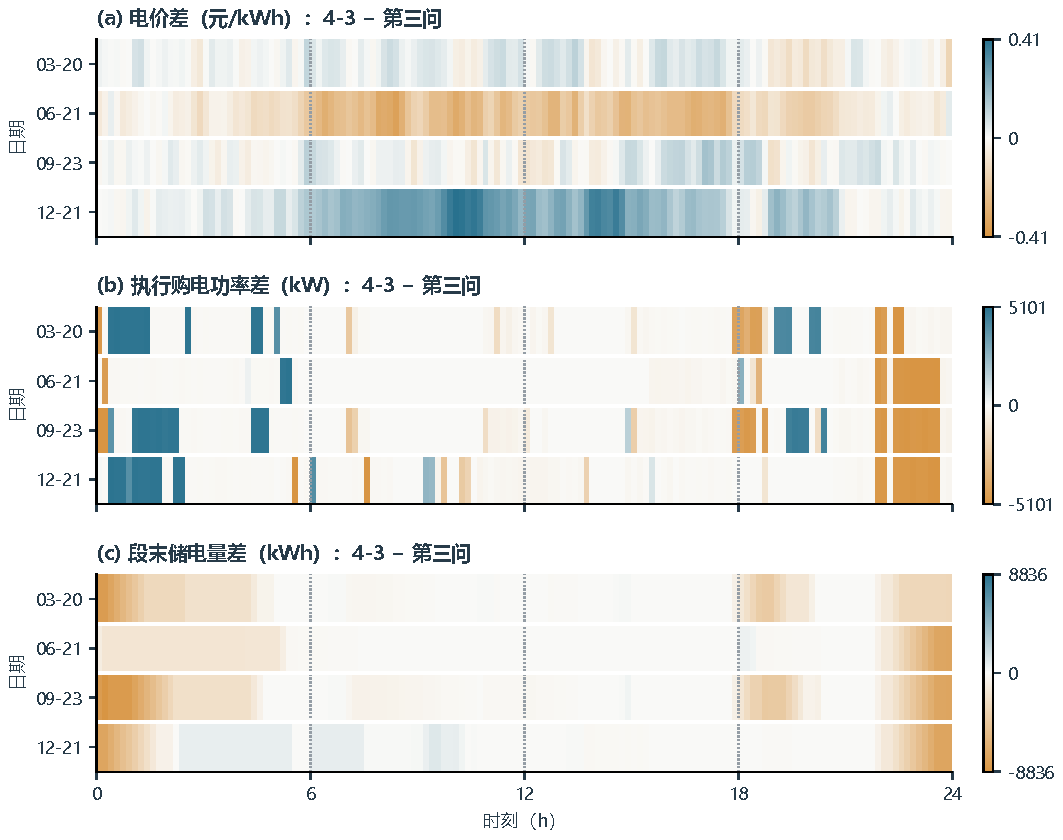
\includegraphics[width=0.95\textwidth]{10_q43_schedule_differences.pdf}
\caption{四个指定日中，4-3 相对第三问的电价、最终执行购电功率及段末储电量差值。
蓝色表示 4-3 更高，橙色表示更低，白色表示接近零；各面板使用独立的对称色标，
数值未裁剪，竖虚线为 6、12、18 点。}
\label{fig:q43-diff}
\end{figure}

配对差值图保留了两问在相同实际负载与光伏条件下的时段对应关系。
电价、购电与储能状态的差异具有不同的时间分布，显示调度响应包含跨时段的能量转移。
各指定日的初始储电量已由此前滚动执行决定，两问并不相同，
因此状态差异既包含当日决策差异，也包含前期累积影响；
图中比较用于描述两套已保存运行结果，不将某一列的颜色直接解释为另一列的因果效应。

\begin{figure}[H]
\centering
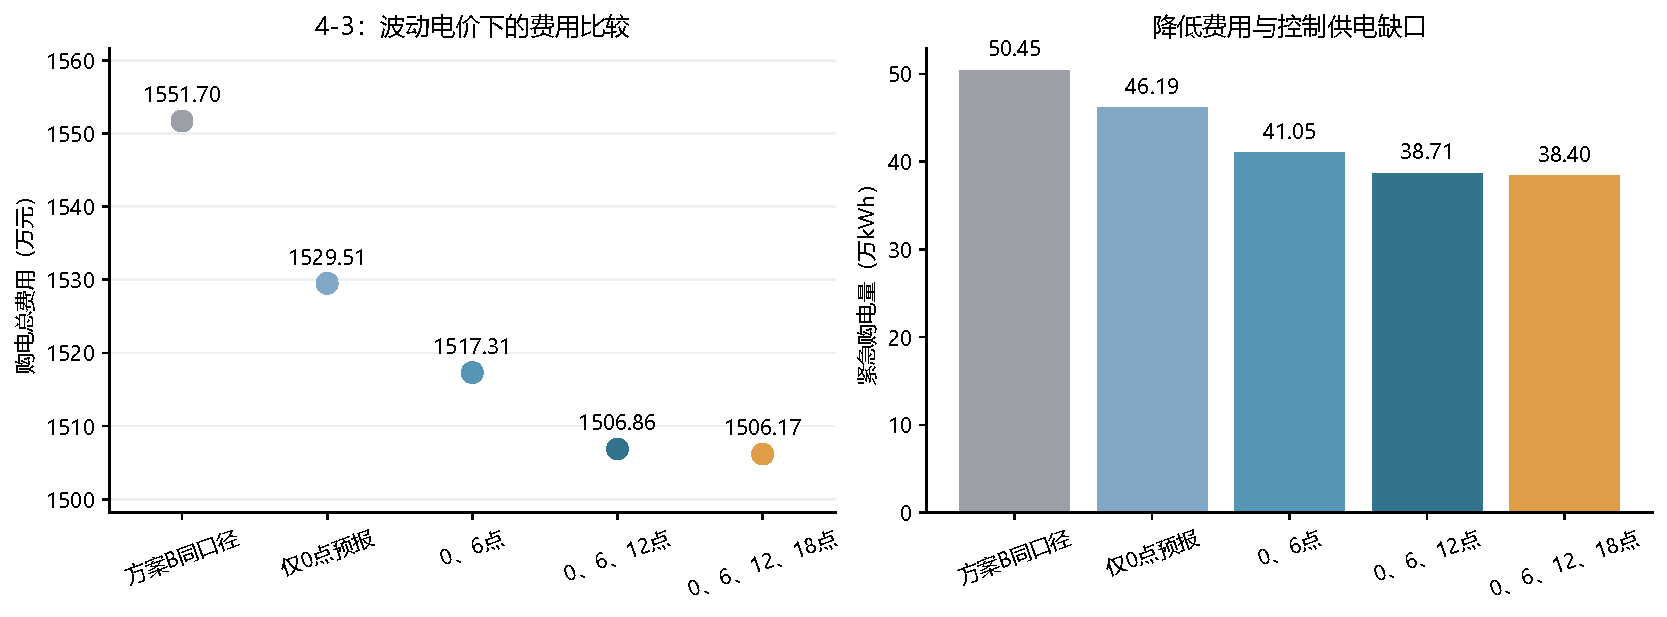
\includegraphics[width=0.9\textwidth]{q43_cost.pdf}
\caption{4-3：各方案费用对照}
\label{fig:q43-cost}
\end{figure}

\begin{figure}[H]
\centering
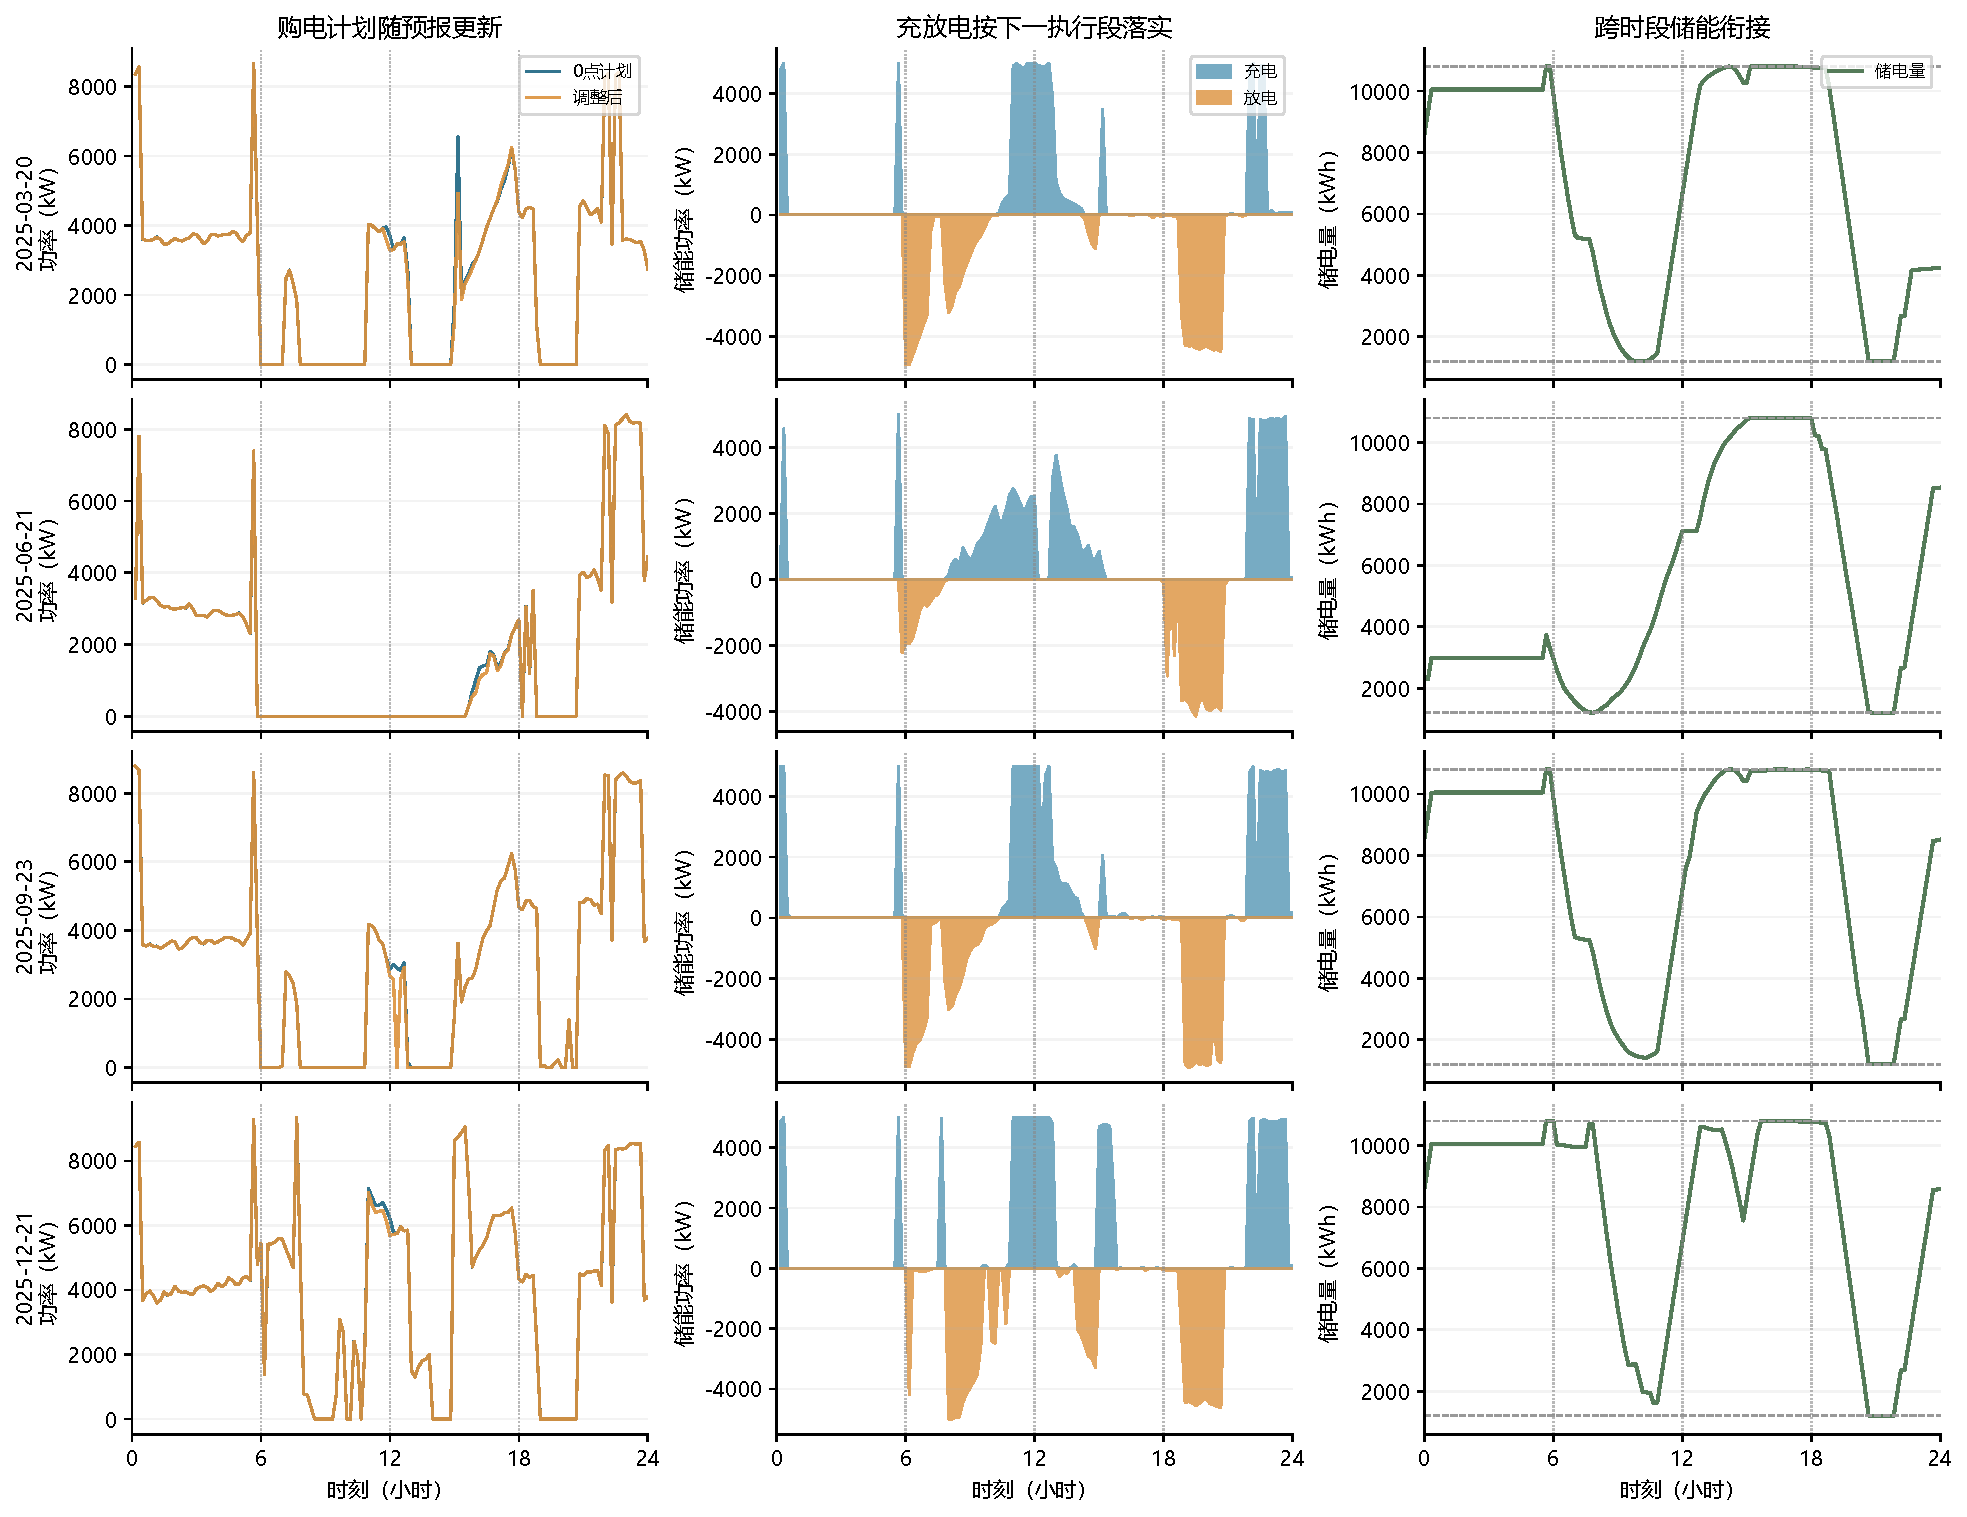
\includegraphics[width=0.9\textwidth]{q43_dispatch.pdf}
\caption{4-3：指定日期的购电与储能调度（波动电价下）}
\label{fig:q43-dispatch}
\end{figure}

\FloatBarrier

% ==================== 七、模型评价与推广 ====================
\section{模型评价与推广}

\subsection{模型优点}

\begin{enumerate}[itemsep=4pt,topsep=4pt]
  \item \textbf{统一而递进的建模框架。}
        四问共享"预测 $\to$ 场景 $\to$ 线性规划 $\to$ 滚动执行"的基本结构，
        并逐层增加不确定性维度（电价已知 $\to$ 负载/光伏未知 $\to$ 多时点信息 $\to$ 电价亦未知）。
        这种设计使得各问之间的差异\textbf{可归因、可对照}，
        避免了"四问四套模型、无法横向比较"的常见问题。

  \item \textbf{报童结构的识别提供了经济学解释。}
        我们把问题二识别为报童模型，导出临界分位 $F^*=0.80$，
        说明"计划量应取 80\% 分位而非均值"。
        这使参数设定有理论依据，而非依赖盲目试错；
        也解释了为何早期"按点预测制定计划"的方案会产生大量昂贵的紧急购电。

  \item \textbf{LP 松弛紧性的严格证明（问题一）。}
        用等 SOC 扰动证明：在往返效率 $0.81<1$ 且该时段有购电的前提下，
        同时充放电必劣于拆开。由此\textbf{无需二元变量}，
        问题规模保持在线性规划量级，而 LP 与 MILP 数值结果完全一致
        （$35\,126.95$ 元，差 $0.000000$），证明了推导的正确性。

  \item \textbf{非前视由变量结构保证。}
        问题三的场景树中，同一节点内的所有场景\textbf{共享同一组控制变量}，
        使模型在结构上不可能"针对已知场景分别决策"。
        这比仅添加额外约束更为稳健，也便于审阅者验证。

  \item \textbf{电价—净负载联合场景的正确性论证。}
        我们指出 $\E[p\cdot(N-z)_+]\neq\E[p]\E[(N-z)_+]$，
        并据此采用同历史日配对的场景构造，保留了"高电价与缺电同时发生"的风险耦合。

  \item \textbf{严格的因果性与可复现性。}
        所有预测与融合权重均只使用决策时刻之前的数据；
        程序对 $48\,096$ 个时段逐段核验能量平衡、效率递推、SOC 边界、功率上限、
        互斥性、跨日连续、初末状态、缺口与费用，并反读 Excel 输出。
    \item \textbf{诚实的对照报告。}
        所有未胜出的方案（半衰期加权、短窗口、在线选窗、平均电价模型、
        多源信息、$k$ 参数扫描等）均在结果与附录中保留，
        便于审阅者评估结论的稳健性。
\end{enumerate}

\subsection{模型局限}

\begin{enumerate}[itemsep=4pt,topsep=4pt]
  \item \textbf{非全局最优}：本文为有限经验场景上的线性规划加滚动执行，
        不宣称全年真实随机控制问题的全局最优解。
        小型二叉场景树、次日确定性近似、反复滚动重算都是对真实问题的近似。

  \item \textbf{结果均为同年回测}：所有费用数字来自 2025 年 2--12 月的滚动回测，
        不证明在其他年份仍最优。例如问题三中"$18$ 点更新无收益"是本年度数据结论。

  \item \textbf{预测内核参数的选型过程未完全审计}：
        负载的"最近 4 次同星期 $+$ 近 5 日漂移"、光伏的"近 7 日 $+$ 近 28 日漂移"
        等参数继承自前期研发，
        本次因果性检查只能验证"运行时未使用未来数据"，
        不能证明当初的参数选择未使用过测试年份信息。

  \item \textbf{题面若干处的建模解释需公开声明}：
        问题三"取消部分退原价、另付 50\% 违约费"是本文采用的结算解释；
        若改为"不退原价、另罚 50\%"，则同一调度方案的费用会变化，
        且应重新优化而非仅调整报表公式。该敏感性已写入核验文件。

  \item \textbf{储能模型简化}：未计入折旧、寿命衰减、温度与功率相关性，
        也未考虑电池的最小充放电持续时间等工程约束。

  \item \textbf{场景样本量受限于历史长度}：2 月 1 日仅 24 条残差样本，
        场景分布的尾部刻画精度有限。
\end{enumerate}

\subsection{模型推广}

\begin{enumerate}[itemsep=3pt,topsep=3pt]
  \item \textbf{引入外部气象数据}。当前光伏预报误差是主要成本来源
        （完美预见下界与现实的差距约 $179$ 万元）；
        引入辐照度、云量、温度等特征，或按天气类型分别建模，
        有望显著降低预报误差。

  \item \textbf{自适应场景树深度}。当前固定 4 层、15 节点，
        可依据样本量与预报修订的方差结构自适应确定分支深度，
        在样本充足时提供更细的信息分辨率。

  \item \textbf{电价预测的增强}。可引入电价曲线的日内形状聚类、
        天气耦合与节假日效应，改善 4-2/4-3 中电价预测的精度
        （该误差对应约 $1.0\%$ 的费用）。

  \item \textbf{储能全寿命周期成本建模}。加入循环次数与放电深度的折旧模型，
        可避免"为套利而过度循环"的短视调度。

  \item \textbf{多微网协同}。若扩展至多微网共享储能或互联互济，
        本文的场景树框架可直接推广为多主体随机博弈结构。
\end{enumerate}


\newpage
% ==================== 八、参考文献 ====================
\renewcommand{\refname}{参考文献}
\begin{thebibliography}{99}
\setlength{\itemsep}{2pt}

\bibitem{newsvendor}
Porteus E L. Foundations of Stochastic Inventory Theory.
Stanford University Press, 2002. （报童模型与临界分位）

\bibitem{birge}
Birge J R, Louveaux F. Introduction to Stochastic Programming.
2nd ed. Springer, 2011. （两阶段与多阶段随机规划）

\bibitem{kall}
Kall P, Wallace S W. Stochastic Programming. Wiley, 1994.
（场景树、非前视约束与信息分支）

\bibitem{scenred}
Dupačová J, Gröwe-Kuska N, Römisch W. Scenario reduction in stochastic programming:
an approach using probability metrics. Mathematical Programming, 2003, 95(3): 493--511.

\bibitem{rhs}
Dontchev A L, Hager W W, Veliov V M. Second-order Runge-Kutta approximations in
control constrained optimal control. SIAM Journal on Numerical Analysis, 2000, 38(1): 202--226.
（滚动时域优化与终端条件的作用）

\bibitem{highs}
Huangfu Q, Hall J A J. Parallelizing the dual revised simplex method.
Mathematical Programming Computation, 2018, 10(1): 119--142. （HiGHS 求解器）

\bibitem{scipy}
Virtanen P, Gommers R, Oliphant T E, et al. SciPy 1.0: fundamental algorithms for
scientific computing in Python. Nature Methods, 2020, 17: 261--272.

\bibitem{microgrid}
王成山, 武震, 李鹏. 微电网关键技术研究. 电工技术学报, 2014, 29(2): 1--12.

\bibitem{storage}
陈吕鹏, 潘毅, 王超. 微电网储能系统容量优化配置与运行策略研究综述.
电力系统自动化, 2018, 42(19): 188--199.

\bibitem{pvforecast}
Antonanzas J, Osorio N, Escobar R, et al. Review of photovoltaic power forecasting.
Solar Energy, 2016, 136: 78--111. （光伏预报方法与误差特性）

\bibitem{priceforecast}
Weron R. Electricity price forecasting: a review of the state-of-the-art with a look
into the future. International Journal of Forecasting, 2014, 30(4): 1030--1081.

\bibitem{fusion}
Bates J M, Granger C W J. The combination of forecasts.
Operational Research Quarterly, 1969, 20(4): 451--468. （预报融合与最优权重）

\end{thebibliography}


\newpage
% ==================== 附录 ====================
\appendix
\renewcommand{\thesection}{附录 \Alph{section}}
\section{支撑材料文件列表}

本次提交的支撑材料为文件夹 \texttt{final\_version/}（压缩为单个文件提交），
其内容与下表的对应关系如下。
所有源程序均为完整、可直接运行版本，运行环境见 \S\ref{sec:appendix-env}。

\begin{table}[H]
\centering
\footnotesize
\setlength{\tabcolsep}{4pt}
\caption{支撑材料文件列表（\texttt{final\_version/} 目录结构）}
\label{tab:appendix-files}
\begin{tabularx}{\textwidth}{@{}l X c@{}}
\toprule
路径 & 说明 & 对应问题 \\
\midrule
\multicolumn{3}{@{}l}{\textbf{一、源程序}} \\
\midrule
\texttt{Q1/q1\_code/}      & \texttt{q1\_model.py} 数据读取与 LP/MILP 建模、约束核验、对偶量；\texttt{run\_q1.py} 主流程与导出；\texttt{plot\_q1.py} 绘图 & 问题一 \\
\midrule
\texttt{Q2/code/}          & \texttt{rolling\_window.py} 有效残差与候选窗口；\texttt{run\_experiment.py} 滚动执行；\texttt{verify\_window.py}、\texttt{check\_information.py} 核验；\texttt{report\_experiment.py} 汇总发布；\texttt{make\_target\_tables.py} 题目要求表 & 问题二 \\
\midrule
\texttt{Q3/code/}          & \texttt{q3\_data.py} 输入校验；\texttt{q3\_forecast.py} 预报融合；\texttt{q3\_model.py} 场景树 LP；\texttt{run\_q3.py} 滚动执行；\texttt{verify\_q3.py} 核验；\texttt{plot\_q3.py} 绘图 & 问题三 \\
\midrule
\texttt{Q4/part2/code/}    & \texttt{q42\_model.py} 电价预测与联合场景；\texttt{run\_q42.py} 主流程；\texttt{report\_q42.py} 汇总；\texttt{verify\_q42.py}、\texttt{check\_information.py} 核验 & 问题四-2 \\
\midrule
\texttt{Q4/part3/code/}    & 在问题三代码基础上增加实时电价场景与结算；\texttt{requirements.txt} 依赖清单 & 问题四-3 \\
\midrule
\texttt{common/q2\_base/}  & 第二问与 4-2 共用的基础 LP 与数据层（\texttt{q2\_data.py}、\texttt{run\_1439.py}） & 二 / 四 \\
\texttt{common/efficiency/} & \texttt{template\_layout.py} 附件5 结果模板表头（主程序读取模板所必需） & 一 / 二 / 三 / 四 \\
\texttt{common/plotting/}  & \texttt{setup\_style.py}、\texttt{export\_figure.py} 统一绘图样式与导出 & 全部 \\
\midrule
\multicolumn{3}{@{}l}{\textbf{二、结果与图表}} \\
\midrule
\texttt{Q1..Q4/*/results/} & \texttt{result*.xlsx} 正式结果（题目要求格式）、\texttt{summary.json} 汇总指标、\texttt{schedule\_detail.csv} 逐时段明细、\texttt{verification.json} 核验记录、\texttt{figures/} 插图源文件 & 全部 \\
\texttt{Q2/results/variants/}、\texttt{Q2/results/extensions/}、\texttt{Q2/results/sensitivity/} & 各候选窗口方案、短窗口扩展与敏感性分析的完整对照结果 & 问题二 \\
\texttt{Q3/results/comparisons/} & 四种发布时点方案（\texttt{B\_aligned}、\texttt{only\_0}、\texttt{at\_0\_6}、\texttt{at\_0\_6\_12}）的完整结果 & 问题三 \\
\texttt{Q4/part2/results/}、\texttt{Q4/part3/results/} & 各电价场景方案与指定日的完整结果 & 问题四 \\
\midrule
\multicolumn{3}{@{}l}{\textbf{三、数据}} \\
\midrule
\texttt{data/附件/}        & \texttt{附件1--4.xlsx} 原始数据；\texttt{附件5/} 结果文件模板（\texttt{result1.xlsx} 等 5 个） & 全部 \\
\bottomrule
\end{tabularx}
\end{table}

\textbf{说明}：\texttt{final\_version/} 为自包含目录，解压后无需任何外部文件
即可按 \S\ref{sec:appendix-env} 的命令复现全部结果；
附录 \S\ref{sec:appendix-source} 的源程序\textbf{直接取自该目录}，
与所提交文件逐字一致。

\section{运行环境与复现方法}
\label{sec:appendix-env}

\begin{table}[H]
\centering
\small
\caption{软件环境}
\begin{tabularx}{\textwidth}{@{}l X@{}}
\toprule
项目 & 版本 / 说明 \\
\midrule
操作系统 & Windows \\
Python   & 3.12 / 3.13 \\
数值计算 & \texttt{numpy}、\texttt{scipy}（HiGHS 求解器）\\
数据处理 & \texttt{pandas}、\texttt{openpyxl}\\
绘图     & \texttt{matplotlib} \\
论文排版 & XeLaTeX $+$ \texttt{ctex}（中文支持）\\
\bottomrule
\end{tabularx}
\end{table}

\textbf{复现步骤}（在 \texttt{final\_version/} 目录下执行）：

\begin{verbatim}
python -m pip install -r Q4/part3/requirements.txt

# 问题一
python -X utf8 Q1/q1_code/run_q1.py

# 问题二（推荐方案：有效残差 + 56 天等权）
python -X utf8 Q2/code/run_experiment.py \
       --first-residual 7 --only uniform56 --out recommended_only
python -X utf8 Q2/code/make_target_tables.py     # 题目要求的表1/表2/表3

# 问题三（四次更新主方案）
python -X utf8 Q3/code/run_q3.py --mode all --out reproduced
python -X utf8 Q3/code/verify_q3.py              # 独立核验

# 问题四
python -X utf8 Q4/part2/code/run_q42.py --primary joint_price
python -X utf8 Q4/part3/code/run_q3.py --mode all --out out
python -X utf8 Q4/part3/code/verify_q3.py        # 独立核验
\end{verbatim}

\textbf{说明}：
\begin{itemize}[itemsep=2pt,topsep=3pt]
  \item 各脚本内部路径均相对于文件位置，从任意工作目录用脚本绝对路径启动均可。
  \item 问题二\textbf{无参数默认运行的是原始残差口径候选}，
        不是最终推荐方案，须按上述命令显式指定 \texttt{--first-residual 7}。
  \item 问题四-2 会读取 \texttt{Q2/results/} 下的 Q2 结果作为同口径基准，
        因此需先运行问题二。
  \item 运行主程序会覆盖同名结果文件；论文使用的现有结果应先备份。
\end{itemize}

\section{核验记录摘要}

\begin{table}[H]
\centering
\caption{逐时段核验项目（四问合计 $48\,096$ 段/年）}
\small
\begin{tabular}{@{}l l c@{}}
\toprule
核验项 & 判据 & 结果 \\
\midrule
能量平衡            & $g+V+d=L+c+w$ 残差 $<10^{-9}$ & 通过 \\
效率递推            & $E_t-E_{t-1}-0.9c_t+d_t/0.9=0$ & 通过 \\
SOC 边界            & $1200\le E_t\le10800$ & 通过 \\
充放电功率          & $0\le c_t,d_t\le 833.33\kw$ & 通过 \\
充放电互斥          & $c_t\,d_t=0$（逐段检查）& 通过 \\
跨日连续性          & 相邻日末初电量一致（偏差 $<10^{-9}$）& 通过 \\
初末条件            & 起始/终止电量符合设定 & 通过 \\
实际缺口            & $e_t=\max(N_t-z_t,0)$ & 通过 \\
费用复算            & 独立重算与程序输出一致 & 通过 \\
Excel 反读          & 读回结果文件与内部数组一致 & 通过 \\
非前视（信息扰动）  & 扰动未来数据不改变当前决策 & 通过 \\
\bottomrule
\end{tabular}
\end{table}

\textbf{信息扰动测试的具体做法}（以问题三为例）：
在 2 月 1 日、6 月 21 日、12 月 21 日的四个发布时刻，
\textbf{修改当天及未来的全部实际值与未发布预报}，重建预测、残差、融合权重、场景树与 LP，
检查\textbf{当前的预测结果与控制量是否保持不变}。结果显示决策完全不变，
证明程序未使用任何未来信息。

% 按 data/C题.pdf 第1—3页要求，由各问主结果逐段数据重建。
% 仅作汇总，不调用求解器；六个指定十分钟时段取 slot=60,72,84,96,108,120。
\clearpage
\section{题目指定时段与指定日期结果}
\label{sec:required-results}
本附录按题目表1、表2、表3的字段列示五组主结果。电量单位为kWh，费用单位为元；
十分钟时段按起止时刻定位，四小时充放电由连续24段累计，紧急购电按连续发生区间汇总。
第三问与4-3同时列出0点原计划和最终调整后购电，实际总费用包括计划费、净调整费及紧急费。
下列金额和电量由未舍入数据汇总后保留两位小数，舍入后的分项相加可能相差0.01。

\subsection{问题一}
\begin{table}[H]
\centering\footnotesize
\setlength{\tabcolsep}{4pt}
\caption{问题一：指定时段购电及全天汇总（题表1，电量单位：kWh）}
\label{tab:required-q1-grid}
\begin{tabular}{@{}lrlrlr@{}}
\toprule
时间段 & 购电量 & 时间段 & 购电量 & 时间段 & 购电量 \\
\midrule
10:00--10:10 & 0.00 & 12:00--12:10 & 480.41 & 14:00--14:10 & 0.00 \\
16:00--16:10 & 445.43 & 18:00--18:10 & 531.89 & 20:00--20:10 & 0.00 \\
\multicolumn{2}{l}{全天购电量} & 59482.70 & \multicolumn{2}{l}{全天购电费（元）} & 35126.95 \\
\bottomrule
\end{tabular}
\end{table}

\begin{table}[H]
\centering\footnotesize
\setlength{\tabcolsep}{4pt}
\caption{问题一：指定时段充放电及首末储电量（题表2，单位：kWh）}
\label{tab:required-q1-storage}
\begin{tabular}{@{}lrrlrr@{}}
\toprule
时间段 & 充电量 & 放电量 & 时间段 & 充电量 & 放电量 \\
\midrule
00:00--04:00 & 4500.00 & 0.00 & 04:00--08:00 & 833.33 & 6365.84 \\
08:00--12:00 & 4787.96 & 1703.00 & 12:00--16:00 & 5286.04 & 91.10 \\
16:00--20:00 & 0.00 & 5780.13 & 20:00--24:00 & 5333.33 & 2859.87 \\
\multicolumn{2}{l}{0:00储电量} & 6000.00 & \multicolumn{2}{l}{24:00储电量} & 6000.00 \\
\bottomrule
\end{tabular}
\end{table}

\clearpage
\subsection{问题二}
\begin{table}[H]
\centering\footnotesize
\setlength{\tabcolsep}{4pt}
\caption{问题二 2025-03-20：指定时段购电及全天汇总（题表1，电量单位：kWh）}
\label{tab:required-q2-2025-03-20-grid}
\begin{tabular}{@{}lrlrlr@{}}
\toprule
时间段 & 购电量 & 时间段 & 购电量 & 时间段 & 购电量 \\
\midrule
10:00--10:10 & 0.00 & 12:00--12:10 & 626.63 & 14:00--14:10 & 0.00 \\
16:00--16:10 & 494.24 & 18:00--18:10 & 706.68 & 20:00--20:10 & 0.00 \\
\multicolumn{2}{l}{全天计划购电量} & 65615.94 & \multicolumn{2}{l}{计划购电费（元）} & 40493.15 \\
\multicolumn{2}{l}{全天紧急购电量} & 689.80 & \multicolumn{2}{l}{紧急购电费（元）} & 2775.85 \\
\multicolumn{5}{l}{全天总购电费（元）} & 43269.00 \\
\bottomrule
\end{tabular}
\end{table}

\begin{table}[H]
\centering\footnotesize
\setlength{\tabcolsep}{4pt}
\caption{问题二 2025-03-20：指定时段充放电及首末储电量（题表2，单位：kWh）}
\label{tab:required-q2-2025-03-20-storage}
\begin{tabular}{@{}lrrlrr@{}}
\toprule
时间段 & 充电量 & 放电量 & 时间段 & 充电量 & 放电量 \\
\midrule
00:00--04:00 & 1666.67 & 0.00 & 04:00--08:00 & 833.33 & 5501.23 \\
08:00--12:00 & 5912.26 & 3138.77 & 12:00--16:00 & 5454.26 & 566.88 \\
16:00--20:00 & 0.00 & 5671.59 & 20:00--24:00 & 3498.06 & 2968.41 \\
\multicolumn{2}{l}{0:00储电量} & 8550.00 & \multicolumn{2}{l}{24:00储电量} & 4348.26 \\
\bottomrule
\end{tabular}
\end{table}

\FloatBarrier
\begin{table}[H]
\centering\footnotesize
\setlength{\tabcolsep}{4pt}
\caption{问题二 2025-06-21：指定时段购电及全天汇总（题表1，电量单位：kWh）}
\label{tab:required-q2-2025-06-21-grid}
\begin{tabular}{@{}lrlrlr@{}}
\toprule
时间段 & 购电量 & 时间段 & 购电量 & 时间段 & 购电量 \\
\midrule
10:00--10:10 & 0.00 & 12:00--12:10 & 0.00 & 14:00--14:10 & 0.00 \\
16:00--16:10 & 250.70 & 18:00--18:10 & 0.00 & 20:00--20:10 & 0.00 \\
\multicolumn{2}{l}{全天计划购电量} & 46473.41 & \multicolumn{2}{l}{计划购电费（元）} & 25454.37 \\
\multicolumn{2}{l}{全天紧急购电量} & 338.71 & \multicolumn{2}{l}{紧急购电费（元）} & 1155.49 \\
\multicolumn{5}{l}{全天总购电费（元）} & 26609.86 \\
\bottomrule
\end{tabular}
\end{table}

\begin{table}[H]
\centering\footnotesize
\setlength{\tabcolsep}{4pt}
\caption{问题二 2025-06-21：指定时段充放电及首末储电量（题表2，单位：kWh）}
\label{tab:required-q2-2025-06-21-storage}
\begin{tabular}{@{}lrrlrr@{}}
\toprule
时间段 & 充电量 & 放电量 & 时间段 & 充电量 & 放电量 \\
\midrule
00:00--04:00 & 2869.46 & 0.00 & 04:00--08:00 & 833.33 & 2615.32 \\
08:00--12:00 & 5087.51 & 0.00 & 12:00--16:00 & 3470.92 & 0.00 \\
16:00--20:00 & 0.00 & 6017.99 & 20:00--24:00 & 8166.67 & 2622.01 \\
\multicolumn{2}{l}{0:00储电量} & 2670.80 & \multicolumn{2}{l}{24:00储电量} & 8550.00 \\
\bottomrule
\end{tabular}
\end{table}

\FloatBarrier
\begin{table}[H]
\centering\footnotesize
\setlength{\tabcolsep}{4pt}
\caption{问题二 2025-09-23：指定时段购电及全天汇总（题表1，电量单位：kWh）}
\label{tab:required-q2-2025-09-23-grid}
\begin{tabular}{@{}lrlrlr@{}}
\toprule
时间段 & 购电量 & 时间段 & 购电量 & 时间段 & 购电量 \\
\midrule
10:00--10:10 & 0.00 & 12:00--12:10 & 549.48 & 14:00--14:10 & 0.00 \\
16:00--16:10 & 548.33 & 18:00--18:10 & 777.56 & 20:00--20:10 & 0.00 \\
\multicolumn{2}{l}{全天计划购电量} & 70464.22 & \multicolumn{2}{l}{计划购电费（元）} & 43599.64 \\
\multicolumn{2}{l}{全天紧急购电量} & 1179.52 & \multicolumn{2}{l}{紧急购电费（元）} & 5122.78 \\
\multicolumn{5}{l}{全天总购电费（元）} & 48722.41 \\
\bottomrule
\end{tabular}
\end{table}

\begin{table}[H]
\centering\footnotesize
\setlength{\tabcolsep}{4pt}
\caption{问题二 2025-09-23：指定时段充放电及首末储电量（题表2，单位：kWh）}
\label{tab:required-q2-2025-09-23-storage}
\begin{tabular}{@{}lrrlrr@{}}
\toprule
时间段 & 充电量 & 放电量 & 时间段 & 充电量 & 放电量 \\
\midrule
00:00--04:00 & 1666.67 & 0.00 & 04:00--08:00 & 833.33 & 5644.61 \\
08:00--12:00 & 6191.30 & 2995.39 & 12:00--16:00 & 4841.85 & 296.85 \\
16:00--20:00 & 0.00 & 5695.38 & 20:00--24:00 & 8166.67 & 2944.62 \\
\multicolumn{2}{l}{0:00储电量} & 8550.00 & \multicolumn{2}{l}{24:00储电量} & 8550.00 \\
\bottomrule
\end{tabular}
\end{table}

\FloatBarrier
\begin{table}[H]
\centering\footnotesize
\setlength{\tabcolsep}{4pt}
\caption{问题二 2025-12-21：指定时段购电及全天汇总（题表1，电量单位：kWh）}
\label{tab:required-q2-2025-12-21-grid}
\begin{tabular}{@{}lrlrlr@{}}
\toprule
时间段 & 购电量 & 时间段 & 购电量 & 时间段 & 购电量 \\
\midrule
10:00--10:10 & 0.00 & 12:00--12:10 & 989.93 & 14:00--14:10 & 0.00 \\
16:00--16:10 & 863.82 & 18:00--18:10 & 719.77 & 20:00--20:10 & 0.00 \\
\multicolumn{2}{l}{全天计划购电量} & 98935.42 & \multicolumn{2}{l}{计划购电费（元）} & 63572.16 \\
\multicolumn{2}{l}{全天紧急购电量} & 559.54 & \multicolumn{2}{l}{紧急购电费（元）} & 1933.80 \\
\multicolumn{5}{l}{全天总购电费（元）} & 65505.96 \\
\bottomrule
\end{tabular}
\end{table}

\begin{table}[H]
\centering\footnotesize
\setlength{\tabcolsep}{4pt}
\caption{问题二 2025-12-21：指定时段充放电及首末储电量（题表2，单位：kWh）}
\label{tab:required-q2-2025-12-21-storage}
\begin{tabular}{@{}lrrlrr@{}}
\toprule
时间段 & 充电量 & 放电量 & 时间段 & 充电量 & 放电量 \\
\midrule
00:00--04:00 & 1666.67 & 0.00 & 04:00--08:00 & 1666.67 & 1508.33 \\
08:00--12:00 & 5833.33 & 7806.67 & 12:00--16:00 & 8241.15 & 2760.33 \\
16:00--20:00 & 0.00 & 5609.57 & 20:00--24:00 & 8166.67 & 3030.43 \\
\multicolumn{2}{l}{0:00储电量} & 8550.00 & \multicolumn{2}{l}{24:00储电量} & 8550.00 \\
\bottomrule
\end{tabular}
\end{table}

\FloatBarrier
\begin{table}[H]
\centering\footnotesize
\setlength{\tabcolsep}{2.5pt}
\caption{问题二：指定日期全部紧急购电区间（题表3，单位：kWh）}
\label{tab:required-q2-emergency}
\begin{tabular}{@{}lrlrlrlr@{}}
\toprule
\multicolumn{2}{c}{2025.03.20} & \multicolumn{2}{c}{2025.06.21} & \multicolumn{2}{c}{2025.09.23} & \multicolumn{2}{c}{2025.12.21} \\
\midrule
时间段 & 购电量 & 时间段 & 购电量 & 时间段 & 购电量 & 时间段 & 购电量 \\
\midrule
00:20--00:30 & 12.39 & 00:20--00:30 & 40.44 & 00:30--01:20 & 22.17 & 01:00--01:20 & 29.05 \\
01:10--01:40 & 37.48 & 01:20--01:30 & 21.10 & 02:00--02:20 & 55.41 & 02:10--02:20 & 0.61 \\
03:00--03:30 & 70.17 & 01:50--02:10 & 13.24 & 03:50--04:00 & 11.95 & 03:00--03:10 & 15.38 \\
04:50--05:10 & 48.10 & 02:50--03:30 & 99.52 & 04:50--05:10 & 34.28 & 03:30--03:50 & 108.42 \\
05:50--06:00 & 7.85 & 18:50--19:10 & 78.17 & 05:40--05:50 & 10.72 & 05:50--06:00 & 8.04 \\
08:50--09:10 & 26.14 & 20:20--20:30 & 15.05 & 06:20--06:30 & 1.78 & 06:10--06:30 & 41.11 \\
11:10--11:20 & 8.27 & 22:00--22:30 & 71.19 & 10:00--10:20 & 13.05 & 10:30--11:30 & 271.92 \\
12:30--12:50 & 26.69 & — & — & 10:50--11:00 & 5.98 & 15:20--15:30 & 13.09 \\
15:30--16:20 & 208.66 & — & — & 14:30--15:20 & 272.38 & 18:40--19:00 & 8.15 \\
16:30--17:20 & 61.84 & — & — & 15:50--16:50 & 147.40 & 19:40--20:10 & 63.76 \\
18:40--19:10 & 73.67 & — & — & 17:30--17:40 & 16.92 & — & — \\
20:00--20:20 & 41.73 & — & — & 18:10--18:50 & 111.43 & — & — \\
21:10--21:30 & 42.68 & — & — & 19:10--19:30 & 45.49 & — & — \\
23:30--23:50 & 24.14 & — & — & 19:50--20:30 & 140.64 & — & — \\
— & — & — & — & 20:50--21:10 & 106.59 & — & — \\
— & — & — & — & 21:20--22:00 & 58.24 & — & — \\
— & — & — & — & 22:20--22:30 & 57.72 & — & — \\
— & — & — & — & 23:10--23:40 & 67.37 & — & — \\
合计 & 689.80 & 合计 & 338.71 & 合计 & 1179.52 & 合计 & 559.54 \\
\bottomrule
\end{tabular}
\end{table}

\FloatBarrier
\clearpage
\subsection{问题三}
\begin{table}[H]
\centering\footnotesize
\setlength{\tabcolsep}{4pt}
\caption{问题三指定日期费用与紧急电量汇总}
\label{tab:q3-target}
\begin{tabular}{@{}lrrrr@{}}
\toprule
日期 & 原计划费（元） & 净调整费（元） & 紧急电量（kWh） & 总费用（元） \\
\midrule
2025-03-20 & 39999.75 & -94.14 & 873.52 & 43286.36 \\
2025-06-21 & 24123.60 & -105.75 & 342.74 & 25202.45 \\
2025-09-23 & 43523.27 & -155.36 & 949.18 & 47566.49 \\
2025-12-21 & 63209.93 & -75.36 & 607.81 & 65090.39 \\
\bottomrule
\end{tabular}
\end{table}

四个指定日期的净调整费\textbf{均为负}，即调整机制在指定日期上均实现了“省违约金”的净收益。
指定日的完整调度见前文图 \ref{fig:q3-adjust}。

\begin{table}[H]
\centering\footnotesize
\setlength{\tabcolsep}{4pt}
\caption{问题三 2025-03-20：指定时段购电及全天汇总（题表1，电量单位：kWh）}
\label{tab:required-q3-2025-03-20-grid}
\begin{tabular}{@{}lrlrlr@{}}
\toprule
时间段 & 购电量 & 时间段 & 购电量 & 时间段 & 购电量 \\
\midrule
\multicolumn{6}{c}{0点原计划购电量} \\
10:00--10:10 & 0.00 & 12:00--12:10 & 551.93 & 14:00--14:10 & 0.00 \\
16:00--16:10 & 544.34 & 18:00--18:10 & 705.08 & 20:00--20:10 & 0.00 \\
\multicolumn{2}{l}{全天计划购电量} & 64668.95 & \multicolumn{2}{l}{计划购电费（元）} & 39999.75 \\
\multicolumn{6}{c}{最终调整后购电量（不含紧急购电）} \\
10:00--10:10 & 0.00 & 12:00--12:10 & 551.93 & 14:00--14:10 & 0.00 \\
16:00--16:10 & 544.34 & 18:00--18:10 & 705.08 & 20:00--20:10 & 0.00 \\
\multicolumn{2}{l}{全天调整后购电量} & 64101.47 & \multicolumn{2}{l}{净调整费（元）} & -94.14 \\
\multicolumn{2}{l}{全天紧急购电量} & 873.52 & \multicolumn{2}{l}{紧急购电费（元）} & 3380.75 \\
\multicolumn{5}{l}{全天总购电费（元）} & 43286.36 \\
\bottomrule
\end{tabular}
\end{table}

\begin{table}[H]
\centering\footnotesize
\setlength{\tabcolsep}{4pt}
\caption{问题三 2025-03-20：指定时段充放电及首末储电量（题表2，单位：kWh）}
\label{tab:required-q3-2025-03-20-storage}
\begin{tabular}{@{}lrrlrr@{}}
\toprule
时间段 & 充电量 & 放电量 & 时间段 & 充电量 & 放电量 \\
\midrule
00:00--04:00 & 1629.40 & 0.00 & 04:00--08:00 & 833.33 & 5973.45 \\
08:00--12:00 & 6049.15 & 2666.55 & 12:00--16:00 & 5195.34 & 468.04 \\
16:00--20:00 & 2.26 & 5675.55 & 20:00--24:00 & 3395.02 & 2974.39 \\
\multicolumn{2}{l}{0:00储电量} & 8583.54 & \multicolumn{2}{l}{24:00储电量} & 4246.51 \\
\bottomrule
\end{tabular}
\end{table}

\FloatBarrier
\begin{table}[H]
\centering\footnotesize
\setlength{\tabcolsep}{4pt}
\caption{问题三 2025-06-21：指定时段购电及全天汇总（题表1，电量单位：kWh）}
\label{tab:required-q3-2025-06-21-grid}
\begin{tabular}{@{}lrlrlr@{}}
\toprule
时间段 & 购电量 & 时间段 & 购电量 & 时间段 & 购电量 \\
\midrule
\multicolumn{6}{c}{0点原计划购电量} \\
10:00--10:10 & 0.00 & 12:00--12:10 & 0.00 & 14:00--14:10 & 0.00 \\
16:00--16:10 & 223.91 & 18:00--18:10 & 0.00 & 20:00--20:10 & 0.00 \\
\multicolumn{2}{l}{全天计划购电量} & 43570.65 & \multicolumn{2}{l}{计划购电费（元）} & 24123.60 \\
\multicolumn{6}{c}{最终调整后购电量（不含紧急购电）} \\
10:00--10:10 & 0.00 & 12:00--12:10 & 0.00 & 14:00--14:10 & 0.00 \\
16:00--16:10 & 176.27 & 18:00--18:10 & 0.00 & 20:00--20:10 & 0.00 \\
\multicolumn{2}{l}{全天调整后购电量} & 43321.19 & \multicolumn{2}{l}{净调整费（元）} & -105.75 \\
\multicolumn{2}{l}{全天紧急购电量} & 342.74 & \multicolumn{2}{l}{紧急购电费（元）} & 1184.60 \\
\multicolumn{5}{l}{全天总购电费（元）} & 25202.45 \\
\bottomrule
\end{tabular}
\end{table}

\begin{table}[H]
\centering\footnotesize
\setlength{\tabcolsep}{4pt}
\caption{问题三 2025-06-21：指定时段充放电及首末储电量（题表2，单位：kWh）}
\label{tab:required-q3-2025-06-21-storage}
\begin{tabular}{@{}lrrlrr@{}}
\toprule
时间段 & 充电量 & 放电量 & 时间段 & 充电量 & 放电量 \\
\midrule
00:00--04:00 & 762.83 & 0.00 & 04:00--08:00 & 857.88 & 2271.65 \\
08:00--12:00 & 6553.33 & 0.00 & 12:00--16:00 & 4083.07 & 0.00 \\
16:00--20:00 & 0.00 & 5995.04 & 20:00--24:00 & 8149.49 & 2645.72 \\
\multicolumn{2}{l}{0:00储电量} & 2292.66 & \multicolumn{2}{l}{24:00储电量} & 8533.70 \\
\bottomrule
\end{tabular}
\end{table}

\FloatBarrier
\begin{table}[H]
\centering\footnotesize
\setlength{\tabcolsep}{4pt}
\caption{问题三 2025-09-23：指定时段购电及全天汇总（题表1，电量单位：kWh）}
\label{tab:required-q3-2025-09-23-grid}
\begin{tabular}{@{}lrlrlr@{}}
\toprule
时间段 & 购电量 & 时间段 & 购电量 & 时间段 & 购电量 \\
\midrule
\multicolumn{6}{c}{0点原计划购电量} \\
10:00--10:10 & 0.00 & 12:00--12:10 & 502.56 & 14:00--14:10 & 0.00 \\
16:00--16:10 & 560.29 & 18:00--18:10 & 767.73 & 20:00--20:10 & 0.00 \\
\multicolumn{2}{l}{全天计划购电量} & 70219.95 & \multicolumn{2}{l}{计划购电费（元）} & 43523.27 \\
\multicolumn{6}{c}{最终调整后购电量（不含紧急购电）} \\
10:00--10:10 & 0.00 & 12:00--12:10 & 430.27 & 14:00--14:10 & 0.00 \\
16:00--16:10 & 560.29 & 18:00--18:10 & 767.73 & 20:00--20:10 & 0.00 \\
\multicolumn{2}{l}{全天调整后购电量} & 69537.44 & \multicolumn{2}{l}{净调整费（元）} & -155.36 \\
\multicolumn{2}{l}{全天紧急购电量} & 949.18 & \multicolumn{2}{l}{紧急购电费（元）} & 4198.58 \\
\multicolumn{5}{l}{全天总购电费（元）} & 47566.49 \\
\bottomrule
\end{tabular}
\end{table}

\begin{table}[H]
\centering\footnotesize
\setlength{\tabcolsep}{4pt}
\caption{问题三 2025-09-23：指定时段充放电及首末储电量（题表2，单位：kWh）}
\label{tab:required-q3-2025-09-23-storage}
\begin{tabular}{@{}lrrlrr@{}}
\toprule
时间段 & 充电量 & 放电量 & 时间段 & 充电量 & 放电量 \\
\midrule
00:00--04:00 & 1682.24 & 0.00 & 04:00--08:00 & 833.33 & 5844.03 \\
08:00--12:00 & 6049.67 & 2598.82 & 12:00--16:00 & 4754.75 & 331.14 \\
16:00--20:00 & 42.16 & 5706.45 & 20:00--24:00 & 8152.71 & 2962.87 \\
\multicolumn{2}{l}{0:00储电量} & 8535.99 & \multicolumn{2}{l}{24:00储电量} & 8517.90 \\
\bottomrule
\end{tabular}
\end{table}

\FloatBarrier
\begin{table}[H]
\centering\footnotesize
\setlength{\tabcolsep}{4pt}
\caption{问题三 2025-12-21：指定时段购电及全天汇总（题表1，电量单位：kWh）}
\label{tab:required-q3-2025-12-21-grid}
\begin{tabular}{@{}lrlrlr@{}}
\toprule
时间段 & 购电量 & 时间段 & 购电量 & 时间段 & 购电量 \\
\midrule
\multicolumn{6}{c}{0点原计划购电量} \\
10:00--10:10 & 0.00 & 12:00--12:10 & 965.84 & 14:00--14:10 & 0.00 \\
16:00--16:10 & 872.53 & 18:00--18:10 & 708.71 & 20:00--20:10 & 0.00 \\
\multicolumn{2}{l}{全天计划购电量} & 98380.06 & \multicolumn{2}{l}{计划购电费（元）} & 63209.93 \\
\multicolumn{6}{c}{最终调整后购电量（不含紧急购电）} \\
10:00--10:10 & 0.00 & 12:00--12:10 & 954.33 & 14:00--14:10 & 0.00 \\
16:00--16:10 & 872.53 & 18:00--18:10 & 708.71 & 20:00--20:10 & 0.00 \\
\multicolumn{2}{l}{全天调整后购电量} & 98056.59 & \multicolumn{2}{l}{净调整费（元）} & -75.36 \\
\multicolumn{2}{l}{全天紧急购电量} & 607.81 & \multicolumn{2}{l}{紧急购电费（元）} & 1955.82 \\
\multicolumn{5}{l}{全天总购电费（元）} & 65090.39 \\
\bottomrule
\end{tabular}
\end{table}

\begin{table}[H]
\centering\footnotesize
\setlength{\tabcolsep}{4pt}
\caption{问题三 2025-12-21：指定时段充放电及首末储电量（题表2，单位：kWh）}
\label{tab:required-q3-2025-12-21-storage}
\begin{tabular}{@{}lrrlrr@{}}
\toprule
时间段 & 充电量 & 放电量 & 时间段 & 充电量 & 放电量 \\
\midrule
00:00--04:00 & 1640.14 & 0.00 & 04:00--08:00 & 1660.82 & 1605.72 \\
08:00--12:00 & 5884.07 & 7358.10 & 12:00--16:00 & 7766.93 & 2767.14 \\
16:00--20:00 & 7.42 & 5602.70 & 20:00--24:00 & 8200.89 & 3043.38 \\
\multicolumn{2}{l}{0:00储电量} & 8573.87 & \multicolumn{2}{l}{24:00储电量} & 8576.96 \\
\bottomrule
\end{tabular}
\end{table}

\FloatBarrier
\begin{table}[H]
\centering\footnotesize
\setlength{\tabcolsep}{2.5pt}
\caption{问题三：指定日期全部紧急购电区间（题表3，单位：kWh）}
\label{tab:required-q3-emergency}
\begin{tabular}{@{}lrlrlrlr@{}}
\toprule
\multicolumn{2}{c}{2025.03.20} & \multicolumn{2}{c}{2025.06.21} & \multicolumn{2}{c}{2025.09.23} & \multicolumn{2}{c}{2025.12.21} \\
\midrule
时间段 & 购电量 & 时间段 & 购电量 & 时间段 & 购电量 & 时间段 & 购电量 \\
\midrule
00:20--00:30 & 12.39 & 00:20--00:30 & 40.44 & 00:30--01:20 & 22.17 & 01:00--01:20 & 29.05 \\
01:10--01:40 & 37.48 & 01:20--01:30 & 21.10 & 02:00--02:20 & 55.41 & 02:10--02:20 & 0.61 \\
03:00--03:30 & 70.17 & 01:50--02:10 & 13.24 & 03:50--04:00 & 11.95 & 03:00--03:10 & 15.38 \\
04:50--05:10 & 48.10 & 02:50--03:30 & 99.52 & 04:50--05:10 & 34.31 & 03:30--03:50 & 108.42 \\
05:50--06:00 & 6.72 & 18:50--19:10 & 79.29 & 05:40--05:50 & 17.70 & 05:50--06:00 & 8.04 \\
08:10--09:20 & 147.65 & 20:20--20:30 & 18.51 & 06:10--06:30 & 0.57 & 06:20--06:30 & 15.63 \\
09:40--10:00 & 56.01 & 22:00--22:30 & 70.63 & 07:40--07:50 & 5.03 & 10:30--11:40 & 363.36 \\
11:00--11:30 & 114.30 & — & — & 14:20--15:00 & 75.47 & 13:00--13:10 & 1.78 \\
11:40--12:00 & 35.27 & — & — & 15:50--16:40 & 126.89 & 18:40--19:00 & 6.49 \\
12:30--12:50 & 109.16 & — & — & 17:30--17:50 & 19.82 & 19:40--20:00 & 59.05 \\
13:10--13:20 & 0.81 & — & — & 18:10--18:50 & 96.87 & — & — \\
14:00--14:10 & 6.50 & — & — & 19:10--19:30 & 41.82 & — & — \\
15:50--16:10 & 22.60 & — & — & 19:50--20:30 & 131.14 & — & — \\
16:50--17:00 & 0.11 & — & — & 20:50--21:10 & 106.59 & — & — \\
18:40--19:10 & 85.04 & — & — & 21:20--22:00 & 78.37 & — & — \\
19:50--20:20 & 49.50 & — & — & 22:20--22:30 & 57.72 & — & — \\
21:10--21:30 & 47.58 & — & — & 23:10--23:40 & 67.37 & — & — \\
23:30--23:50 & 24.14 & — & — & — & — & — & — \\
合计 & 873.52 & 合计 & 342.74 & 合计 & 949.18 & 合计 & 607.81 \\
\bottomrule
\end{tabular}
\end{table}

\FloatBarrier
\clearpage
\subsection{问题四（4-2）}
\begin{table}[H]
\centering\footnotesize
\setlength{\tabcolsep}{4pt}
\caption{问题四（4-2） 2025-03-20：指定时段购电及全天汇总（题表1，电量单位：kWh）}
\label{tab:required-q42-2025-03-20-grid}
\begin{tabular}{@{}lrlrlr@{}}
\toprule
时间段 & 购电量 & 时间段 & 购电量 & 时间段 & 购电量 \\
\midrule
10:00--10:10 & 0.00 & 12:00--12:10 & 653.15 & 14:00--14:10 & 12.32 \\
16:00--16:10 & 494.35 & 18:00--18:10 & 0.00 & 20:00--20:10 & 731.74 \\
\multicolumn{2}{l}{全天计划购电量} & 63984.26 & \multicolumn{2}{l}{计划购电费（元）} & 41035.65 \\
\multicolumn{2}{l}{全天紧急购电量} & 631.45 & \multicolumn{2}{l}{紧急购电费（元）} & 2706.13 \\
\multicolumn{5}{l}{全天总购电费（元）} & 43741.78 \\
\bottomrule
\end{tabular}
\end{table}

\begin{table}[H]
\centering\footnotesize
\setlength{\tabcolsep}{4pt}
\caption{问题四（4-2） 2025-03-20：指定时段充放电及首末储电量（题表2，单位：kWh）}
\label{tab:required-q42-2025-03-20-storage}
\begin{tabular}{@{}lrrlrr@{}}
\toprule
时间段 & 充电量 & 放电量 & 时间段 & 充电量 & 放电量 \\
\midrule
00:00--04:00 & 2500.00 & 0.00 & 04:00--08:00 & 1500.00 & 5904.30 \\
08:00--12:00 & 5922.21 & 3144.53 & 12:00--16:00 & 5058.38 & 520.46 \\
16:00--20:00 & 0.00 & 6405.44 & 20:00--24:00 & 833.33 & 2234.56 \\
\multicolumn{2}{l}{0:00储电量} & 7950.00 & \multicolumn{2}{l}{24:00储电量} & 1950.00 \\
\bottomrule
\end{tabular}
\end{table}

\FloatBarrier
\begin{table}[H]
\centering\footnotesize
\setlength{\tabcolsep}{4pt}
\caption{问题四（4-2） 2025-06-21：指定时段购电及全天汇总（题表1，电量单位：kWh）}
\label{tab:required-q42-2025-06-21-grid}
\begin{tabular}{@{}lrlrlr@{}}
\toprule
时间段 & 购电量 & 时间段 & 购电量 & 时间段 & 购电量 \\
\midrule
10:00--10:10 & 0.00 & 12:00--12:10 & 0.00 & 14:00--14:10 & 0.00 \\
16:00--16:10 & 252.87 & 18:00--18:10 & 487.95 & 20:00--20:10 & 0.00 \\
\multicolumn{2}{l}{全天计划购电量} & 49515.72 & \multicolumn{2}{l}{计划购电费（元）} & 23064.36 \\
\multicolumn{2}{l}{全天紧急购电量} & 311.29 & \multicolumn{2}{l}{紧急购电费（元）} & 1037.19 \\
\multicolumn{5}{l}{全天总购电费（元）} & 24101.55 \\
\bottomrule
\end{tabular}
\end{table}

\begin{table}[H]
\centering\footnotesize
\setlength{\tabcolsep}{4pt}
\caption{问题四（4-2） 2025-06-21：指定时段充放电及首末储电量（题表2，单位：kWh）}
\label{tab:required-q42-2025-06-21-storage}
\begin{tabular}{@{}lrrlrr@{}}
\toprule
时间段 & 充电量 & 放电量 & 时间段 & 充电量 & 放电量 \\
\midrule
00:00--04:00 & 0.00 & 0.00 & 04:00--08:00 & 2749.81 & 2227.34 \\
08:00--12:00 & 7535.00 & 0.00 & 12:00--16:00 & 3131.66 & 0.00 \\
16:00--20:00 & 0.00 & 6017.99 & 20:00--24:00 & 9166.67 & 2757.01 \\
\multicolumn{2}{l}{0:00储电量} & 1200.00 & \multicolumn{2}{l}{24:00储电量} & 9300.00 \\
\bottomrule
\end{tabular}
\end{table}

\FloatBarrier
\begin{table}[H]
\centering\footnotesize
\setlength{\tabcolsep}{4pt}
\caption{问题四（4-2） 2025-09-23：指定时段购电及全天汇总（题表1，电量单位：kWh）}
\label{tab:required-q42-2025-09-23-grid}
\begin{tabular}{@{}lrlrlr@{}}
\toprule
时间段 & 购电量 & 时间段 & 购电量 & 时间段 & 购电量 \\
\midrule
10:00--10:10 & 0.00 & 12:00--12:10 & 568.09 & 14:00--14:10 & 0.00 \\
16:00--16:10 & 550.06 & 18:00--18:10 & 0.00 & 20:00--20:10 & 0.00 \\
\multicolumn{2}{l}{全天计划购电量} & 70272.43 & \multicolumn{2}{l}{计划购电费（元）} & 45565.16 \\
\multicolumn{2}{l}{全天紧急购电量} & 1064.22 & \multicolumn{2}{l}{紧急购电费（元）} & 4972.92 \\
\multicolumn{5}{l}{全天总购电费（元）} & 50538.08 \\
\bottomrule
\end{tabular}
\end{table}

\begin{table}[H]
\centering\footnotesize
\setlength{\tabcolsep}{4pt}
\caption{问题四（4-2） 2025-09-23：指定时段充放电及首末储电量（题表2，单位：kWh）}
\label{tab:required-q42-2025-09-23-storage}
\begin{tabular}{@{}lrrlrr@{}}
\toprule
时间段 & 充电量 & 放电量 & 时间段 & 充电量 & 放电量 \\
\midrule
00:00--04:00 & 4166.67 & 0.00 & 04:00--08:00 & 833.33 & 5614.15 \\
08:00--12:00 & 6150.98 & 3025.85 & 12:00--16:00 & 4882.17 & 296.85 \\
16:00--20:00 & 0.00 & 6245.22 & 20:00--24:00 & 4833.33 & 2394.78 \\
\multicolumn{2}{l}{0:00储电量} & 6300.00 & \multicolumn{2}{l}{24:00储电量} & 5550.00 \\
\bottomrule
\end{tabular}
\end{table}

\FloatBarrier
\begin{table}[H]
\centering\footnotesize
\setlength{\tabcolsep}{4pt}
\caption{问题四（4-2） 2025-12-21：指定时段购电及全天汇总（题表1，电量单位：kWh）}
\label{tab:required-q42-2025-12-21-grid}
\begin{tabular}{@{}lrlrlr@{}}
\toprule
时间段 & 购电量 & 时间段 & 购电量 & 时间段 & 购电量 \\
\midrule
10:00--10:10 & 0.00 & 12:00--12:10 & 993.19 & 14:00--14:10 & 0.00 \\
16:00--16:10 & 863.82 & 18:00--18:10 & 719.77 & 20:00--20:10 & 0.00 \\
\multicolumn{2}{l}{全天计划购电量} & 97387.54 & \multicolumn{2}{l}{计划购电费（元）} & 74053.41 \\
\multicolumn{2}{l}{全天紧急购电量} & 526.64 & \multicolumn{2}{l}{紧急购电费（元）} & 2403.13 \\
\multicolumn{5}{l}{全天总购电费（元）} & 76456.54 \\
\bottomrule
\end{tabular}
\end{table}

\begin{table}[H]
\centering\footnotesize
\setlength{\tabcolsep}{4pt}
\caption{问题四（4-2） 2025-12-21：指定时段充放电及首末储电量（题表2，单位：kWh）}
\label{tab:required-q42-2025-12-21-storage}
\begin{tabular}{@{}lrrlrr@{}}
\toprule
时间段 & 充电量 & 放电量 & 时间段 & 充电量 & 放电量 \\
\midrule
00:00--04:00 & 666.67 & 0.00 & 04:00--08:00 & 0.00 & 833.33 \\
08:00--12:00 & 5833.33 & 7806.67 & 12:00--16:00 & 8256.22 & 2772.54 \\
16:00--20:00 & 0.00 & 5609.30 & 20:00--24:00 & 8333.33 & 3030.70 \\
\multicolumn{2}{l}{0:00储电量} & 10200.00 & \multicolumn{2}{l}{24:00储电量} & 8700.00 \\
\bottomrule
\end{tabular}
\end{table}

\FloatBarrier
\begin{table}[H]
\centering\footnotesize
\setlength{\tabcolsep}{2.5pt}
\caption{问题四（4-2）：指定日期全部紧急购电区间（题表3，单位：kWh）}
\label{tab:required-q42-emergency}
\begin{tabular}{@{}lrlrlrlr@{}}
\toprule
\multicolumn{2}{c}{2025.03.20} & \multicolumn{2}{c}{2025.06.21} & \multicolumn{2}{c}{2025.09.23} & \multicolumn{2}{c}{2025.12.21} \\
\midrule
时间段 & 购电量 & 时间段 & 购电量 & 时间段 & 购电量 & 时间段 & 购电量 \\
\midrule
00:20--00:30 & 10.64 & 00:20--00:30 & 36.51 & 00:30--00:50 & 10.00 & 01:00--01:20 & 26.83 \\
01:10--01:40 & 32.72 & 01:20--01:30 & 16.72 & 01:00--01:10 & 5.36 & 03:00--03:10 & 13.56 \\
03:00--03:30 & 67.32 & 02:00--02:10 & 10.40 & 02:00--02:20 & 52.79 & 03:30--03:50 & 103.82 \\
04:50--05:10 & 47.52 & 02:50--03:30 & 90.63 & 03:50--04:00 & 9.70 & 05:50--06:00 & 4.79 \\
05:50--06:00 & 6.72 & 18:50--19:10 & 78.17 & 04:50--05:10 & 31.67 & 06:10--06:30 & 34.39 \\
09:00--09:10 & 17.38 & 20:20--20:30 & 15.05 & 05:40--05:50 & 7.01 & 10:30--11:30 & 259.80 \\
12:30--12:50 & 3.28 & 22:00--22:30 & 63.81 & 10:00--10:20 & 4.62 & 15:20--15:30 & 11.52 \\
15:30--16:20 & 199.58 & — & — & 14:30--15:20 & 260.90 & 18:40--19:00 & 8.15 \\
16:30--17:20 & 61.32 & — & — & 15:50--16:50 & 122.31 & 19:40--20:10 & 63.76 \\
18:40--19:10 & 78.09 & — & — & 17:30--17:40 & 16.92 & — & — \\
20:00--20:20 & 43.60 & — & — & 18:10--18:50 & 96.79 & — & — \\
21:10--21:30 & 40.07 & — & — & 19:10--19:30 & 41.85 & — & — \\
23:30--23:50 & 23.20 & — & — & 19:50--20:30 & 140.17 & — & — \\
— & — & — & — & 20:50--21:10 & 105.01 & — & — \\
— & — & — & — & 21:20--22:00 & 54.90 & — & — \\
— & — & — & — & 22:20--22:30 & 57.72 & — & — \\
— & — & — & — & 23:10--23:40 & 46.50 & — & — \\
合计 & 631.45 & 合计 & 311.29 & 合计 & 1064.22 & 合计 & 526.64 \\
\bottomrule
\end{tabular}
\end{table}

\FloatBarrier
\clearpage
\subsection{问题四（4-3）}
\begin{table}[H]
\centering\footnotesize
\setlength{\tabcolsep}{4pt}
\caption{问题四（4-3） 2025-03-20：指定时段购电及全天汇总（题表1，电量单位：kWh）}
\label{tab:required-q43-2025-03-20-grid}
\begin{tabular}{@{}lrlrlr@{}}
\toprule
时间段 & 购电量 & 时间段 & 购电量 & 时间段 & 购电量 \\
\midrule
\multicolumn{6}{c}{0点原计划购电量} \\
10:00--10:10 & 0.00 & 12:00--12:10 & 545.41 & 14:00--14:10 & 0.00 \\
16:00--16:10 & 525.49 & 18:00--18:10 & 0.00 & 20:00--20:10 & 719.50 \\
\multicolumn{2}{l}{全天计划购电量} & 67104.27 & \multicolumn{2}{l}{计划购电费（元）} & 41826.94 \\
\multicolumn{6}{c}{最终调整后购电量（不含紧急购电）} \\
10:00--10:10 & 0.00 & 12:00--12:10 & 545.41 & 14:00--14:10 & 0.00 \\
16:00--16:10 & 525.49 & 18:00--18:10 & 0.00 & 20:00--20:10 & 719.50 \\
\multicolumn{2}{l}{全天调整后购电量} & 66322.18 & \multicolumn{2}{l}{净调整费（元）} & -164.65 \\
\multicolumn{2}{l}{全天紧急购电量} & 1936.99 & \multicolumn{2}{l}{紧急购电费（元）} & 7681.69 \\
\multicolumn{5}{l}{全天总购电费（元）} & 49343.99 \\
\bottomrule
\end{tabular}
\end{table}

\begin{table}[H]
\centering\footnotesize
\setlength{\tabcolsep}{4pt}
\caption{问题四（4-3） 2025-03-20：指定时段充放电及首末储电量（题表2，单位：kWh）}
\label{tab:required-q43-2025-03-20-storage}
\begin{tabular}{@{}lrrlrr@{}}
\toprule
时间段 & 充电量 & 放电量 & 时间段 & 充电量 & 放电量 \\
\midrule
00:00--04:00 & 7500.00 & 0.00 & 04:00--08:00 & 3166.67 & 6274.00 \\
08:00--12:00 & 5993.55 & 2366.00 & 12:00--16:00 & 5097.01 & 343.95 \\
16:00--20:00 & 0.73 & 7170.36 & 20:00--24:00 & 65.10 & 1522.37 \\
\multicolumn{2}{l}{0:00储电量} & 1200.00 & \multicolumn{2}{l}{24:00储电量} & 1200.00 \\
\bottomrule
\end{tabular}
\end{table}

\FloatBarrier
\begin{table}[H]
\centering\footnotesize
\setlength{\tabcolsep}{4pt}
\caption{问题四（4-3） 2025-06-21：指定时段购电及全天汇总（题表1，电量单位：kWh）}
\label{tab:required-q43-2025-06-21-grid}
\begin{tabular}{@{}lrlrlr@{}}
\toprule
时间段 & 购电量 & 时间段 & 购电量 & 时间段 & 购电量 \\
\midrule
\multicolumn{6}{c}{0点原计划购电量} \\
10:00--10:10 & 0.00 & 12:00--12:10 & 0.00 & 14:00--14:10 & 0.00 \\
16:00--16:10 & 192.84 & 18:00--18:10 & 453.05 & 20:00--20:10 & 0.00 \\
\multicolumn{2}{l}{全天计划购电量} & 34666.48 & \multicolumn{2}{l}{计划购电费（元）} & 17225.37 \\
\multicolumn{6}{c}{最终调整后购电量（不含紧急购电）} \\
10:00--10:10 & 0.00 & 12:00--12:10 & 0.00 & 14:00--14:10 & 0.00 \\
16:00--16:10 & 134.07 & 18:00--18:10 & 453.05 & 20:00--20:10 & 0.00 \\
\multicolumn{2}{l}{全天调整后购电量} & 34353.81 & \multicolumn{2}{l}{净调整费（元）} & -93.39 \\
\multicolumn{2}{l}{全天紧急购电量} & 659.63 & \multicolumn{2}{l}{紧急购电费（元）} & 2033.32 \\
\multicolumn{5}{l}{全天总购电费（元）} & 19165.30 \\
\bottomrule
\end{tabular}
\end{table}

\begin{table}[H]
\centering\footnotesize
\setlength{\tabcolsep}{4pt}
\caption{问题四（4-3） 2025-06-21：指定时段充放电及首末储电量（题表2，单位：kWh）}
\label{tab:required-q43-2025-06-21-storage}
\begin{tabular}{@{}lrrlrr@{}}
\toprule
时间段 & 充电量 & 放电量 & 时间段 & 充电量 & 放电量 \\
\midrule
00:00--04:00 & 0.00 & 0.00 & 04:00--08:00 & 2586.28 & 2075.00 \\
08:00--12:00 & 6553.33 & 0.00 & 12:00--16:00 & 4107.81 & 15.41 \\
16:00--20:00 & 0.00 & 6096.96 & 20:00--24:00 & 53.86 & 2586.67 \\
\multicolumn{2}{l}{0:00储电量} & 1200.00 & \multicolumn{2}{l}{24:00储电量} & 1200.00 \\
\bottomrule
\end{tabular}
\end{table}

\FloatBarrier
\begin{table}[H]
\centering\footnotesize
\setlength{\tabcolsep}{4pt}
\caption{问题四（4-3） 2025-09-23：指定时段购电及全天汇总（题表1，电量单位：kWh）}
\label{tab:required-q43-2025-09-23-grid}
\begin{tabular}{@{}lrlrlr@{}}
\toprule
时间段 & 购电量 & 时间段 & 购电量 & 时间段 & 购电量 \\
\midrule
\multicolumn{6}{c}{0点原计划购电量} \\
10:00--10:10 & 0.00 & 12:00--12:10 & 456.65 & 14:00--14:10 & 0.00 \\
16:00--16:10 & 536.21 & 18:00--18:10 & 0.00 & 20:00--20:10 & 0.00 \\
\multicolumn{2}{l}{全天计划购电量} & 66826.12 & \multicolumn{2}{l}{计划购电费（元）} & 43138.23 \\
\multicolumn{6}{c}{最终调整后购电量（不含紧急购电）} \\
10:00--10:10 & 0.00 & 12:00--12:10 & 306.14 & 14:00--14:10 & 0.00 \\
16:00--16:10 & 536.21 & 18:00--18:10 & 0.00 & 20:00--20:10 & 0.00 \\
\multicolumn{2}{l}{全天调整后购电量} & 66054.20 & \multicolumn{2}{l}{净调整费（元）} & -57.05 \\
\multicolumn{2}{l}{全天紧急购电量} & 2121.28 & \multicolumn{2}{l}{紧急购电费（元）} & 9624.84 \\
\multicolumn{5}{l}{全天总购电费（元）} & 52706.02 \\
\bottomrule
\end{tabular}
\end{table}

\begin{table}[H]
\centering\footnotesize
\setlength{\tabcolsep}{4pt}
\caption{问题四（4-3） 2025-09-23：指定时段充放电及首末储电量（题表2，单位：kWh）}
\label{tab:required-q43-2025-09-23-storage}
\begin{tabular}{@{}lrrlrr@{}}
\toprule
时间段 & 充电量 & 放电量 & 时间段 & 充电量 & 放电量 \\
\midrule
00:00--04:00 & 7333.33 & 0.00 & 04:00--08:00 & 3333.33 & 6441.96 \\
08:00--12:00 & 6025.31 & 2198.04 & 12:00--16:00 & 4936.43 & 245.51 \\
16:00--20:00 & 25.85 & 6307.45 & 20:00--24:00 & 16.57 & 2360.41 \\
\multicolumn{2}{l}{0:00储电量} & 1200.00 & \multicolumn{2}{l}{24:00储电量} & 1200.00 \\
\bottomrule
\end{tabular}
\end{table}

\FloatBarrier
\begin{table}[H]
\centering\footnotesize
\setlength{\tabcolsep}{4pt}
\caption{问题四（4-3） 2025-12-21：指定时段购电及全天汇总（题表1，电量单位：kWh）}
\label{tab:required-q43-2025-12-21-grid}
\begin{tabular}{@{}lrlrlr@{}}
\toprule
时间段 & 购电量 & 时间段 & 购电量 & 时间段 & 购电量 \\
\midrule
\multicolumn{6}{c}{0点原计划购电量} \\
10:00--10:10 & 0.00 & 12:00--12:10 & 918.26 & 14:00--14:10 & 0.00 \\
16:00--16:10 & 843.15 & 18:00--18:10 & 703.41 & 20:00--20:10 & 0.00 \\
\multicolumn{2}{l}{全天计划购电量} & 95873.43 & \multicolumn{2}{l}{计划购电费（元）} & 72035.15 \\
\multicolumn{6}{c}{最终调整后购电量（不含紧急购电）} \\
10:00--10:10 & 0.00 & 12:00--12:10 & 918.26 & 14:00--14:10 & 0.00 \\
16:00--16:10 & 844.01 & 18:00--18:10 & 703.41 & 20:00--20:10 & 0.00 \\
\multicolumn{2}{l}{全天调整后购电量} & 95320.49 & \multicolumn{2}{l}{净调整费（元）} & -205.31 \\
\multicolumn{2}{l}{全天紧急购电量} & 1295.96 & \multicolumn{2}{l}{紧急购电费（元）} & 5831.56 \\
\multicolumn{5}{l}{全天总购电费（元）} & 77661.40 \\
\bottomrule
\end{tabular}
\end{table}

\begin{table}[H]
\centering\footnotesize
\setlength{\tabcolsep}{4pt}
\caption{问题四（4-3） 2025-12-21：指定时段充放电及首末储电量（题表2，单位：kWh）}
\label{tab:required-q43-2025-12-21-storage}
\begin{tabular}{@{}lrrlrr@{}}
\toprule
时间段 & 充电量 & 放电量 & 时间段 & 充电量 & 放电量 \\
\midrule
00:00--04:00 & 10666.67 & 0.00 & 04:00--08:00 & 3.60 & 864.86 \\
08:00--12:00 & 5833.33 & 7351.09 & 12:00--16:00 & 7885.43 & 2899.17 \\
16:00--20:00 & 12.56 & 5655.47 & 20:00--24:00 & 44.62 & 3030.85 \\
\multicolumn{2}{l}{0:00储电量} & 1200.00 & \multicolumn{2}{l}{24:00储电量} & 1200.00 \\
\bottomrule
\end{tabular}
\end{table}

\FloatBarrier
\begin{table}[H]
\centering\footnotesize
\setlength{\tabcolsep}{2.5pt}
\caption{问题四（4-3）：指定日期全部紧急购电区间（题表3，单位：kWh）}
\label{tab:required-q43-emergency}
\begin{tabular}{@{}lrlrlrlr@{}}
\toprule
\multicolumn{2}{c}{2025.03.20} & \multicolumn{2}{c}{2025.06.21} & \multicolumn{2}{c}{2025.09.23} & \multicolumn{2}{c}{2025.12.21} \\
\midrule
时间段 & 购电量 & 时间段 & 购电量 & 时间段 & 购电量 & 时间段 & 购电量 \\
\midrule
00:20--00:30 & 22.46 & 00:10--00:30 & 74.72 & 00:30--01:20 & 111.02 & 00:00--00:20 & 7.92 \\
01:00--02:00 & 82.55 & 01:20--02:20 & 123.00 & 01:40--02:30 & 112.37 & 01:00--01:20 & 57.62 \\
02:30--02:40 & 0.58 & 02:50--03:30 & 149.65 & 03:40--04:00 & 34.84 & 01:30--01:40 & 11.18 \\
03:00--03:40 & 111.77 & 03:50--04:10 & 13.90 & 04:50--05:20 & 67.28 & 02:10--02:20 & 15.66 \\
04:50--05:20 & 81.18 & 17:20--17:40 & 14.78 & 05:30--05:50 & 29.41 & 02:40--02:50 & 0.88 \\
05:50--06:00 & 20.46 & 18:50--19:10 & 105.08 & 06:10--06:30 & 28.01 & 03:00--03:20 & 37.48 \\
06:40--07:00 & 7.10 & 20:20--20:40 & 52.87 & 06:50--07:10 & 12.98 & 03:30--03:50 & 144.79 \\
08:00--09:20 & 342.10 & 21:40--22:40 & 125.64 & 07:40--08:00 & 26.75 & 04:00--04:20 & 11.40 \\
09:40--10:00 & 80.43 & — & — & 09:30--09:50 & 23.79 & 05:40--06:30 & 97.47 \\
10:20--10:30 & 17.89 & — & — & 10:00--10:20 & 7.35 & 07:10--07:20 & 3.74 \\
10:50--12:00 & 461.66 & — & — & 10:40--11:00 & 35.51 & 07:50--08:00 & 2.03 \\
12:30--13:30 & 191.60 & — & — & 11:30--11:50 & 22.71 & 08:30--09:00 & 24.22 \\
14:00--14:20 & 35.44 & — & — & 12:50--13:00 & 0.16 & 09:30--09:50 & 39.29 \\
14:50--15:00 & 7.47 & — & — & 13:50--14:00 & 14.31 & 10:20--11:50 & 574.75 \\
15:30--16:20 & 90.12 & — & — & 14:20--15:20 & 217.15 & 12:00--12:20 & 39.04 \\
16:40--17:00 & 27.47 & — & — & 15:50--16:50 & 263.19 & 12:40--13:10 & 63.72 \\
18:40--19:20 & 127.95 & — & — & 17:00--17:50 & 73.03 & 15:20--15:30 & 5.86 \\
19:30--20:20 & 93.09 & — & — & 18:00--18:50 & 195.57 & 16:20--16:30 & 11.34 \\
21:10--21:40 & 75.12 & — & — & 19:10--19:30 & 82.27 & 18:00--18:20 & 11.27 \\
23:30--23:50 & 60.55 & — & — & 19:50--22:00 & 562.42 & 18:40--19:00 & 30.66 \\
— & — & — & — & 22:10--22:40 & 77.99 & 19:40--20:10 & 88.22 \\
— & — & — & — & 23:10--23:40 & 123.17 & 21:50--22:00 & 2.84 \\
— & — & — & — & — & — & 22:50--23:00 & 12.06 \\
— & — & — & — & — & — & 23:30--23:40 & 2.50 \\
合计 & 1936.99 & 合计 & 659.63 & 合计 & 2121.28 & 合计 & 1295.96 \\
\bottomrule
\end{tabular}
\end{table}

\FloatBarrier


% ==================== 附录：完整可运行源程序 ====================
% 按 format2026 第五条要求，附录包含建模所用到的完整、可运行的源程序。
% 本文件由 scripts/gen_appendix_source.py 自动生成，勿手改。
% 源码直接取自支撑材料文件夹 final_version/，故与所提交文件逐字一致。
\section{建模源程序（完整可运行）}
\label{sec:appendix-source}

以下按问题列出\textbf{生成论文全部数值结果}所需源程序。
这些代码\textbf{直接取自支撑材料文件夹 \texttt{final\_version/}}，
因此与所提交文件\textbf{逐字一致}；
运行环境与复现命令见 \S\ref{sec:appendix-env}。
全部程序使用 Python 语言与 \texttt{numpy}/\texttt{scipy}（HiGHS 求解器），
Excel 读写使用 \texttt{openpyxl}；未使用 SPSS 等需手工交互的软件，
故无交互命令需要单独记录。

\textbf{收录边界}：本文的图表由配图脚本从上述程序保存的结果文件
（\texttt{*.npz}/\texttt{*.csv}）重建，属于表达层，
不参与任何数值计算，也不影响任何结果；
按“仅收录与建模结果直接相关的源程序”的原则，
\texttt{plot\_*.py} 与 \texttt{common/plotting/} 未列入本附录，
其完整文件已随支撑材料一并提交。

\begingroup
\footnotesize
\setlength{\parindent}{0pt}
\setlength{\parskip}{0pt}

\subsection{问题一：确定性调度}

\subsubsection*{q1\_model.py}
\verbatiminput{../final_version/Q1/q1_code/q1_model.py}

\subsubsection*{run\_q1.py}
\verbatiminput{../final_version/Q1/q1_code/run_q1.py}

\subsection{问题二：滚动随机日前调度}

\subsubsection*{rolling\_window.py}
\verbatiminput{../final_version/Q2/code/rolling_window.py}

\subsubsection*{run\_experiment.py}
\verbatiminput{../final_version/Q2/code/run_experiment.py}

\subsubsection*{verify\_window.py}
\verbatiminput{../final_version/Q2/code/verify_window.py}

\subsubsection*{check\_information.py}
\verbatiminput{../final_version/Q2/code/check_information.py}

\subsubsection*{report\_experiment.py}
\verbatiminput{../final_version/Q2/code/report_experiment.py}

\subsubsection*{make\_target\_tables.py}
\verbatiminput{../final_version/Q2/code/make_target_tables.py}

\subsection{问题三：预报融合与场景树多时点调整}

\subsubsection*{q3\_data.py}
\verbatiminput{../final_version/Q3/code/q3_data.py}

\subsubsection*{q3\_forecast.py}
\verbatiminput{../final_version/Q3/code/q3_forecast.py}

\subsubsection*{q3\_model.py}
\verbatiminput{../final_version/Q3/code/q3_model.py}

\subsubsection*{run\_q3.py}
\verbatiminput{../final_version/Q3/code/run_q3.py}

\subsubsection*{verify\_q3.py}
\verbatiminput{../final_version/Q3/code/verify_q3.py}

\subsection{问题四-2：波动电价下的日前调度}

\subsubsection*{q42\_model.py}
\verbatiminput{../final_version/Q4/part2/code/q42_model.py}

\subsubsection*{run\_q42.py}
\verbatiminput{../final_version/Q4/part2/code/run_q42.py}

\subsubsection*{verify\_q42.py}
\verbatiminput{../final_version/Q4/part2/code/verify_q42.py}

\subsubsection*{check\_information.py}
\verbatiminput{../final_version/Q4/part2/code/check_information.py}

\subsubsection*{report\_q42.py}
\verbatiminput{../final_version/Q4/part2/code/report_q42.py}

\subsection{问题四-3：波动电价下的多时点调整}

\subsubsection*{q3\_data.py}
\verbatiminput{../final_version/Q4/part3/code/q3_data.py}

\subsubsection*{q3\_forecast.py}
\verbatiminput{../final_version/Q4/part3/code/q3_forecast.py}

\subsubsection*{q3\_model.py}
\verbatiminput{../final_version/Q4/part3/code/q3_model.py}

\subsubsection*{run\_q3.py}
\verbatiminput{../final_version/Q4/part3/code/run_q3.py}

\subsubsection*{verify\_q3.py}
\verbatiminput{../final_version/Q4/part3/code/verify_q3.py}

\subsection{公共模块：第二问基础数据与 LP（q2\_base）}

\subsubsection*{q2\_data.py}
\verbatiminput{../final_version/common/q2_base/q2_data.py}

\subsubsection*{run\_1439.py}
\verbatiminput{../final_version/common/q2_base/run_1439.py}

\subsection{公共模块：附件5结果模板表头（主程序依赖）}

\subsubsection*{template\_layout.py}
\verbatiminput{../final_version/common/efficiency/template_layout.py}

\endgroup


\end{document}
